\documentclass[conference]{IEEEtran}

\usepackage[pdftex]{graphicx}
\usepackage{graphicx}
\usepackage[backend=biber,bibstyle=numeric,sorting=ynt]{biblatex}
\addbibresource{references.bib}
\usepackage[colorlinks=true, allcolors=blue]{hyperref}
\usepackage{float}
\usepackage{fancyhdr}
\pagestyle{fancy}
\fancyhf{}
\cfoot{\thepage}

\begin{document}

\title{Face Recognition Dataset}

\author{\IEEEauthorblockN{Pedro Sobral - 98491  - (50\%) - sobral@ua.pt,
Eva Bartolomeu - 98513 - (50\%) - evabartolomeu@ua.pt}
\IEEEauthorblockA{Departamento de Eletrónica, Telecomunicações e Informática,
University of Aveiro, Portugal\\
Fundamentos de Aprendizagem Automática
 - Course Instructor: Pétia Georgieva}}
\maketitle

\maketitle

% As a general rule, do not put math, special symbols or citations
% in the abstract or keywords.
\begin{abstract}
The main goal of this project is to apply suitable machine learning algorithms, notably deep learning techniques learned in class to solve a specific data science problem, in this case, models capable of recognize faces. All the data comes from a Kaggle Dataset \cite{dataset}. In this report, we try to obtain the best result of the accuracy of the implemented models.
\end{abstract}

\begin{IEEEkeywords}
Machine Learning, Classification Model, Logistic Regression, SVM, Neural Network, Normalization, Keras, DeepLearning
\end{IEEEkeywords}

\IEEEpeerreviewmaketitle

\section{Introduction}
In the scope of the subject Fundamentals of Automatic Learning, a work was proposed on a problem (of our choice) of machine learning. The goal of this project is to apply suitable machine learning algorithms learned in class or self-learned to solve a specific data science problem (classification, regression, clustering). Represent the results in graphical/table formats and make analysis and conclusions.
We decided to choose project proposal 3, Face Recognition from Olivetti Dataset. This data set can be used to recognize a face. This dataset is splited in two modules. Target data that have 10 different images of a determined face, and the data itself with other 10 images from the same face but different from the target dataset. Our principal objectives are determine a adequate number of principal components, using the PCA and train models to obtain the best results possible. Will be utilized the Convolutional neural network (CNN) deep learning model, this method was learned during the class. This method is a much more sophisticated approach, to do this implementation will be used the Keras library as in the classes.

\section{State of Art}

The article \cite{5276938} presents a new face recognition method that combines the use of Principle Component Analysis (PCA) as a feature extractor and Support Vector Machines (SVMs) as a classifier. The authors claim that the performance of a face recognition system is determined by the accuracy of the feature extraction and classification. In this paper, PCA is used to extract features from the face images and SVMs are used to classify them. The authors evaluated the developed method, finding that recognition based on SVMs outperforms the standard eigenface approach, and that the results have better accuracy with the application of PCA.

The article \cite{8078730} presents a new image classification method that uses a simple Convolutional Neural Network (CNN), and the respective evaluation with data set. The authors analyze the influence of different methods of learning rate set and different optimization algorithms on image classification. CNN proves to be highly effective in image classification tasks.

The article \cite{bhattacharyya2013face} presents a new face recognition method that uses Linear Discriminant Analysis (LDA), and the respective evaluation with data set. The LDA shows a high correct recognition rate for the face recognition problem.

The article \cite{9137850} presents a new face recognition method that utilizes machine learning algorithms and PCA. The authors claim that traditional face recognition methods have difficulty in real-world situations, such as partial facial occlusion, illumination, and posture variations. The proposed method is tested using linear discriminant analysis, multilayer perceptron, Naive Bayes, and support vector machine, and achieves high accuracy results. 

The article \cite{9716171} presents a new face recognition system that uses machine learning classifier algorithms and PCA for feature extraction. The study evaluates seven machine learning algorithms, such as SVM, Decision Tree, K-Nearest Neighbour, Logistic Regression, Naive Bayes, Multi-Layer Perceptron, and CNN for their performance on the Olivetti faces database.

\section{Data Description}

    Face recognition is a technique to identify people by the face characteristics. So our dataset \cite{dataset} have data, in this case face images, taken between april 1992 and april 1994 from 40 different people. Each person have 10 different images with different facial expressions, variying ligthing, facial express and facial detail. There are 400 differente images in the dataset, each image have a size of 64x64 pixels and all images are in the gray scale. Names of 40 people were encoded to an integer from 0 to 39. The dataset  were initially separate between data itself and target data, where target data have 10 images from the each person, although this images are different from the data that we will use to train our models.

    

\section{Data Visualization}

So we start by visualize the content of the dataset, the figure \ref{fig:example_of_data} shows various sifferent faces, and different shots of each face with diferent angles and different facial expressions. As said before all the images are in gray scale.

\begin{figure}[H]
    \centering
    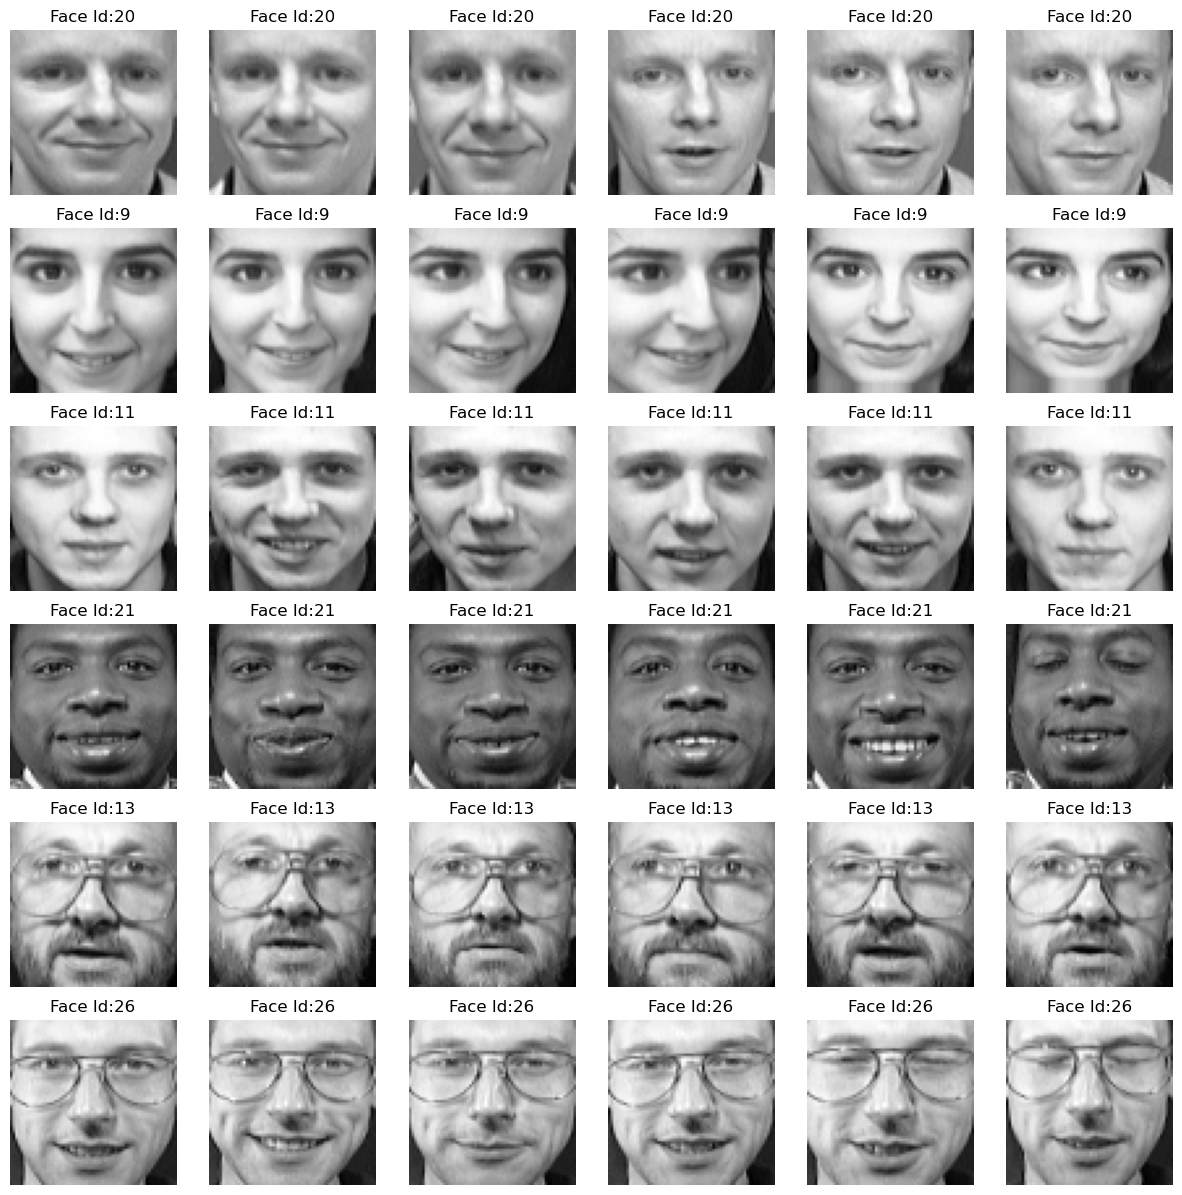
\includegraphics[width=3.8in]{visualization/example_data.png}
    \caption{Example of data from the dataset}
    \label{fig:example_of_data}
\end{figure}

The image data is in matrix form, and before dividing the data into test and training, it is necessary to convert the respective data into a vector.

We decided that 20\% of the data will be used for testing and 80\% of the data will be used for training. For this we created two sets, the test, and the training, using the sklearn.model\_selection.train\_ test\_ split library \cite{train-test-split}.

In order to have deep knowledge about the data-set it is important to have data visualization of the dataset.
The dataset is balanced, this is important so that we have more chance that the model will be certain because the data is well distributed and non-bias. The next figure (Fig. \ref{img:samples_per_class_train}) shows that the number of cases of each class is the same for Training Set.

\begin{figure}[H]
    \centering
    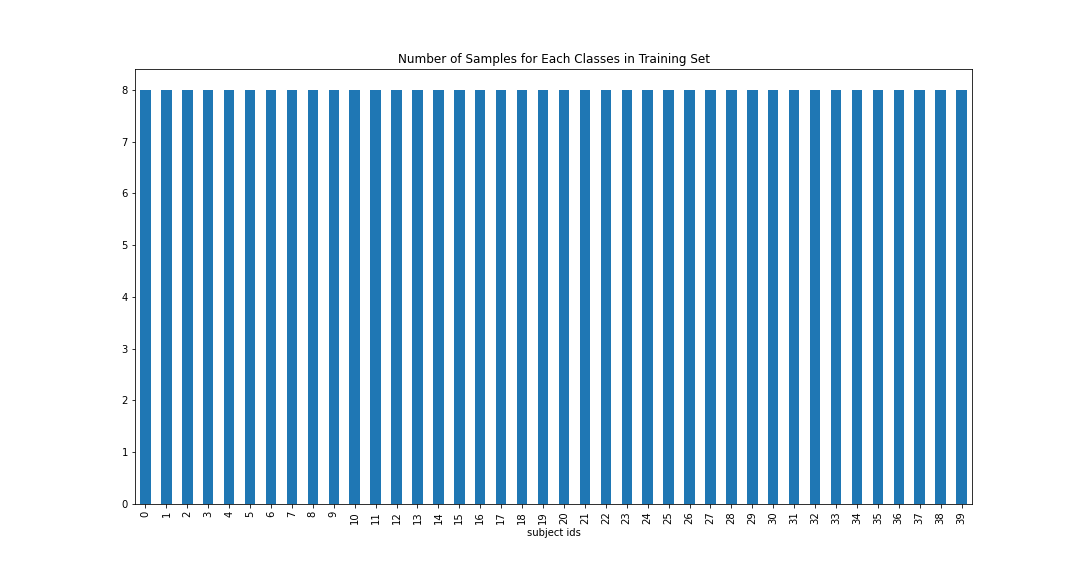
\includegraphics[width=3.8in]{samples_per_class_train.png}
    \caption{Class Distribution in Training Set}
    \label{img:samples_per_class_train}
\end{figure}

The Figure \ref{img:samples_per_class_test.png} also shows that the number of cases of each class is the same for Test Set.

\begin{figure}[H]
    \centering
    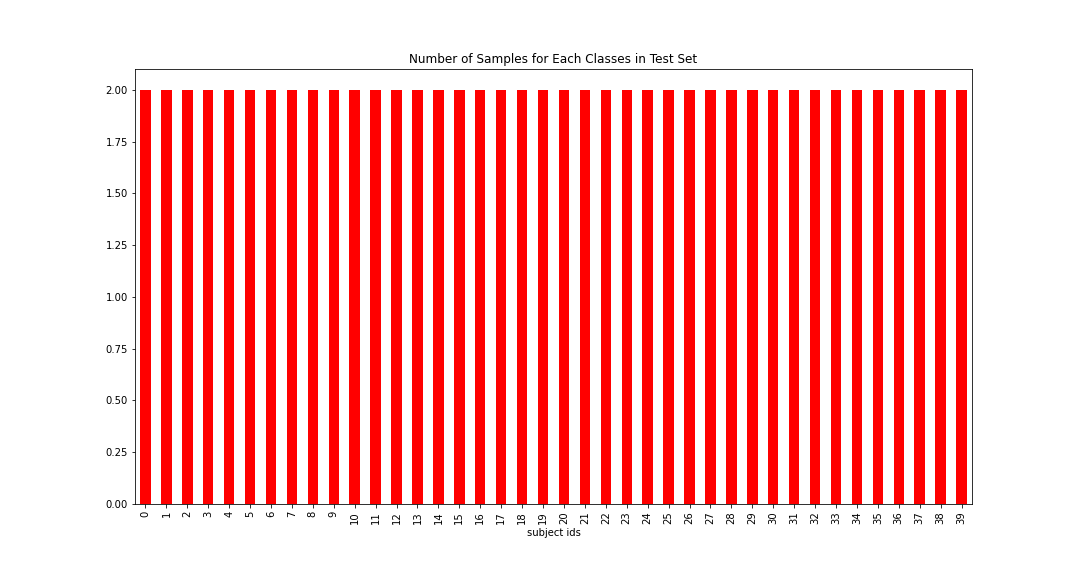
\includegraphics[width=3.8in]{samples_per_class_test.png}
    \caption{Class Distribution in Test Set}
    \label{img:samples_per_class_test.png}
\end{figure}


\section{Data Preprocessing}

As it is a dataset of images, the concept of missing values or outliers is not applicable here. In order to apply a dimension reduction we implement the PCA \cite{pca}, that identifies and discards features that are less useful for making a valid approximation on a dataset. At the same time, to maximise the orthogonality between the features in the transformed feature space.

In order to determine the appropriate number of components for the PCA, we developed a graph that illustrates the trade-off between the number of components used and the amount of information retained in the data after the PCA (Fig. \ref{img:number_of_components_vs_explained_variance.png}).

\begin{figure}[H]
    \centering
    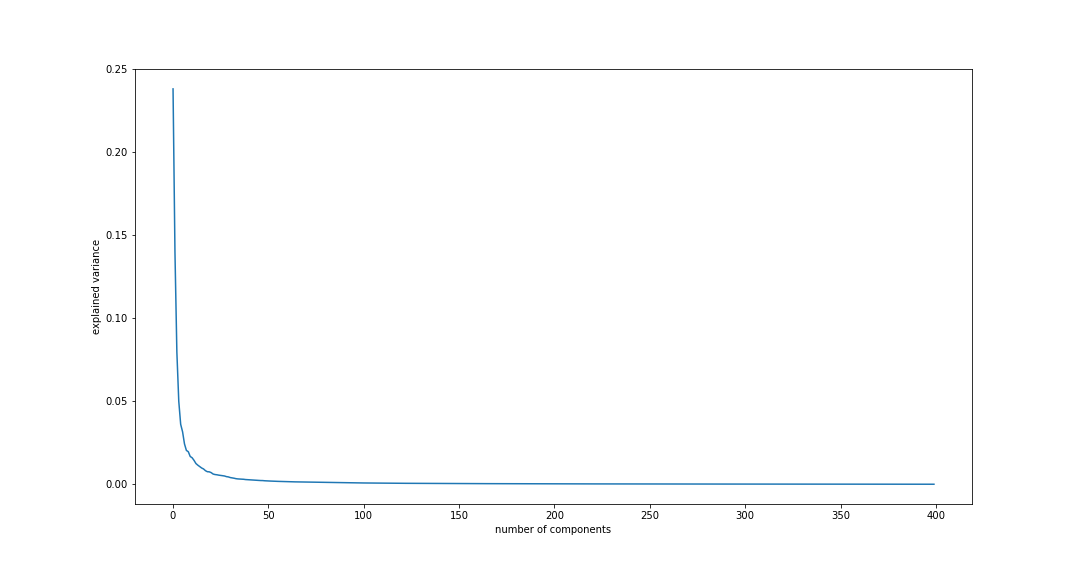
\includegraphics[width=3.8in]{number_of_components_vs_explained_variance.png}
    \caption{Finding Optimum Number of Principle Component}
    \label{img:number_of_components_vs_explained_variance.png}
\end{figure}

Through this graph, we can conclude that the use of more than 50 components does not contribute significantly to the retention of information in the data.

Based on the previous conclusions, we decided to apply the PCA to the training and test sets, using 50 components and with whitening enabled (Fig. \ref{img:pca_of_the_training_set.png} and Fig. \ref{img:pca_of_the_test_set.png}). Whitening is a technique that ensures that the components have zero correlation and unit variance.

\begin{figure}[H]
    \centering
    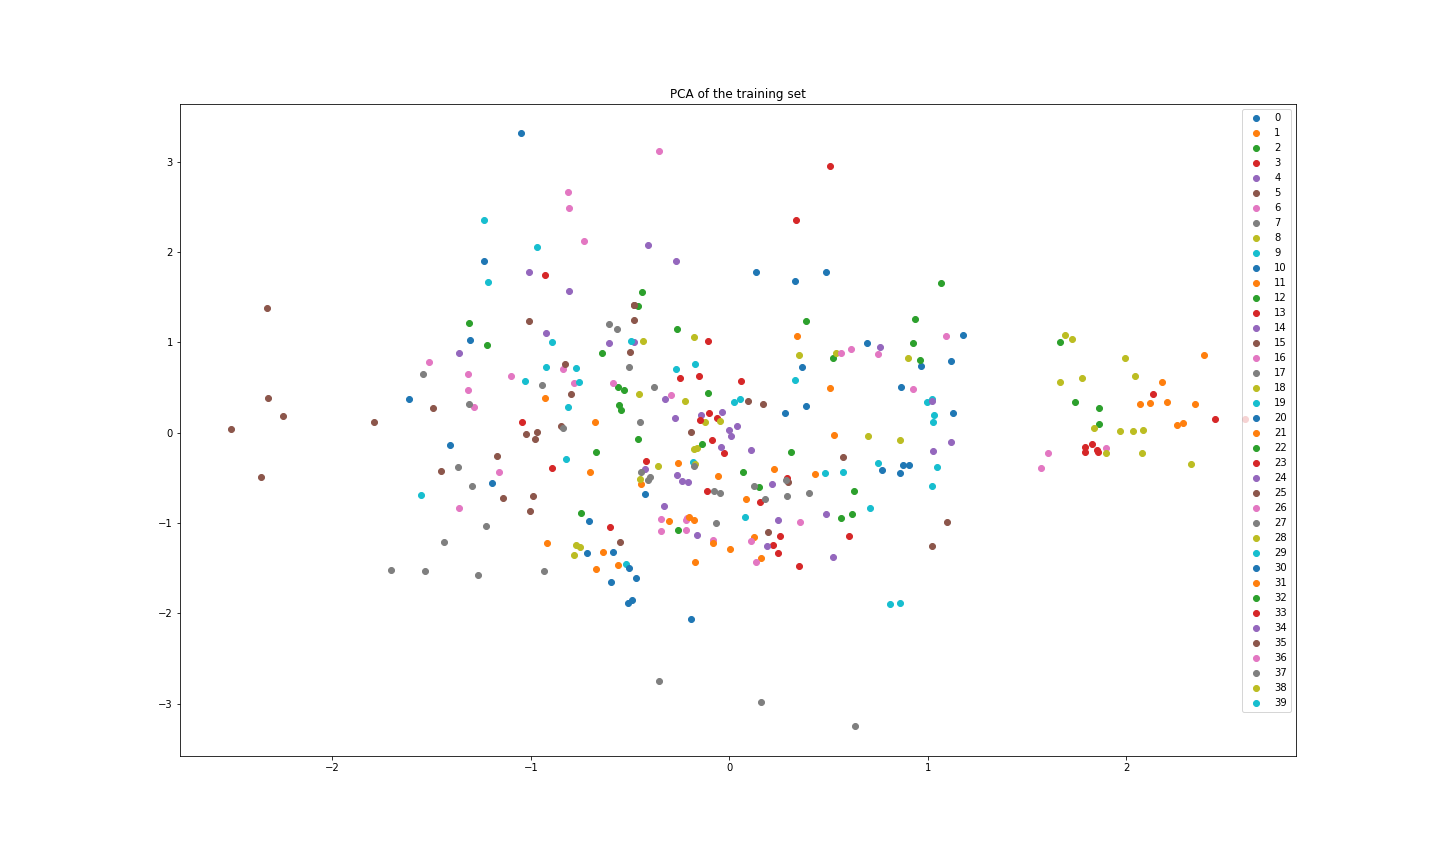
\includegraphics[width=3.8in]{pca_of_the_training_set.png}
    \caption{PCA of the training set}
    \label{img:pca_of_the_training_set.png}
\end{figure}

\begin{figure}[H]
    \centering
    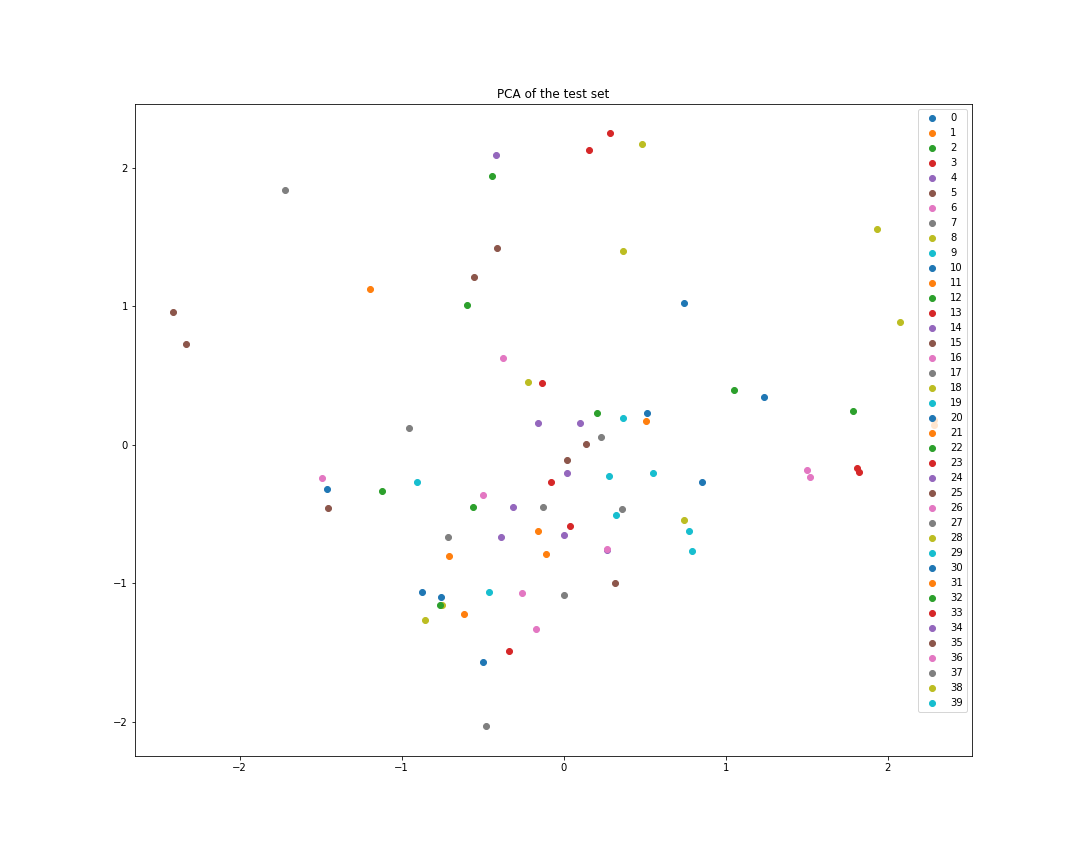
\includegraphics[width=3.8in]{pca_of_the_test_set.png}
    \caption{PCA of the test set}
    \label{img:pca_of_the_test_set.png}
\end{figure}

The sum of all explained variance rates is (~87\%). Graphics of the PCA-transformed sets show that the different classes can be separated by a linear boundary and that the model learned from the training data can generalize well to unseen data.

After PCA, we develop a Average Face image (Fig. \ref{img:mean_face.png}), which is obtained by taking the average of all images in the dataset, reshaping it to the shape of the original image, and displaying it in grayscale. The average face can be used to analyze the general characteristics of the dataset and as a reference to other faces in the dataset.

\begin{figure}[H]
    \centering
    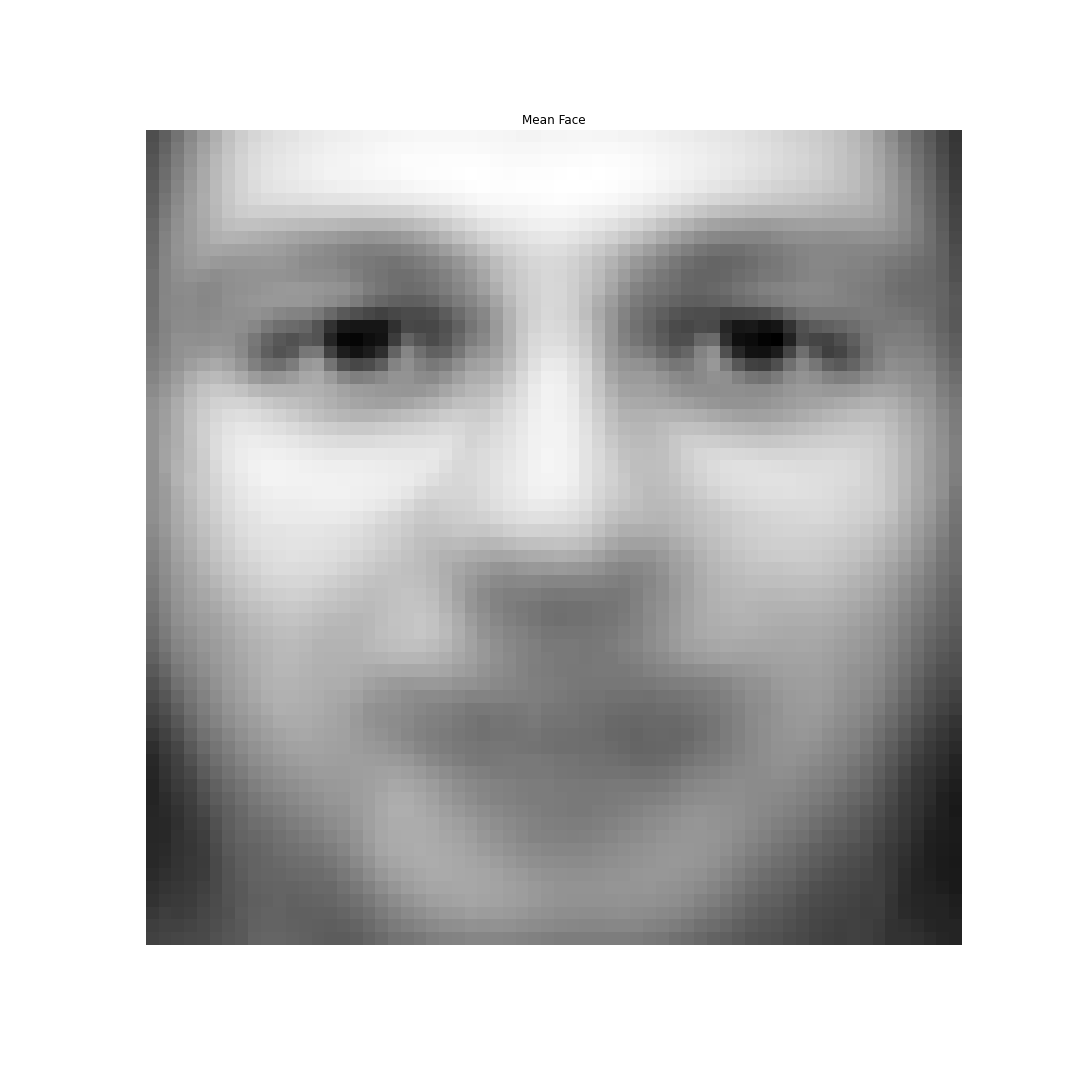
\includegraphics[width=3.0in]{mean_face.png}
    \caption{Average Face after PCA}
    \label{img:mean_face.png}
\end{figure}

Figure \ref{img:eigen_faces.png} presents all the eigenfaces generated by the PCA. Eigenfaces are the main components of the dataset after the PCA and are used to represent the dataset with fewer dimensions. Furthermore, they are linear combinations of the original dataset and are ordered by the amount of variation they represent.

\begin{figure}[H]
    \centering
    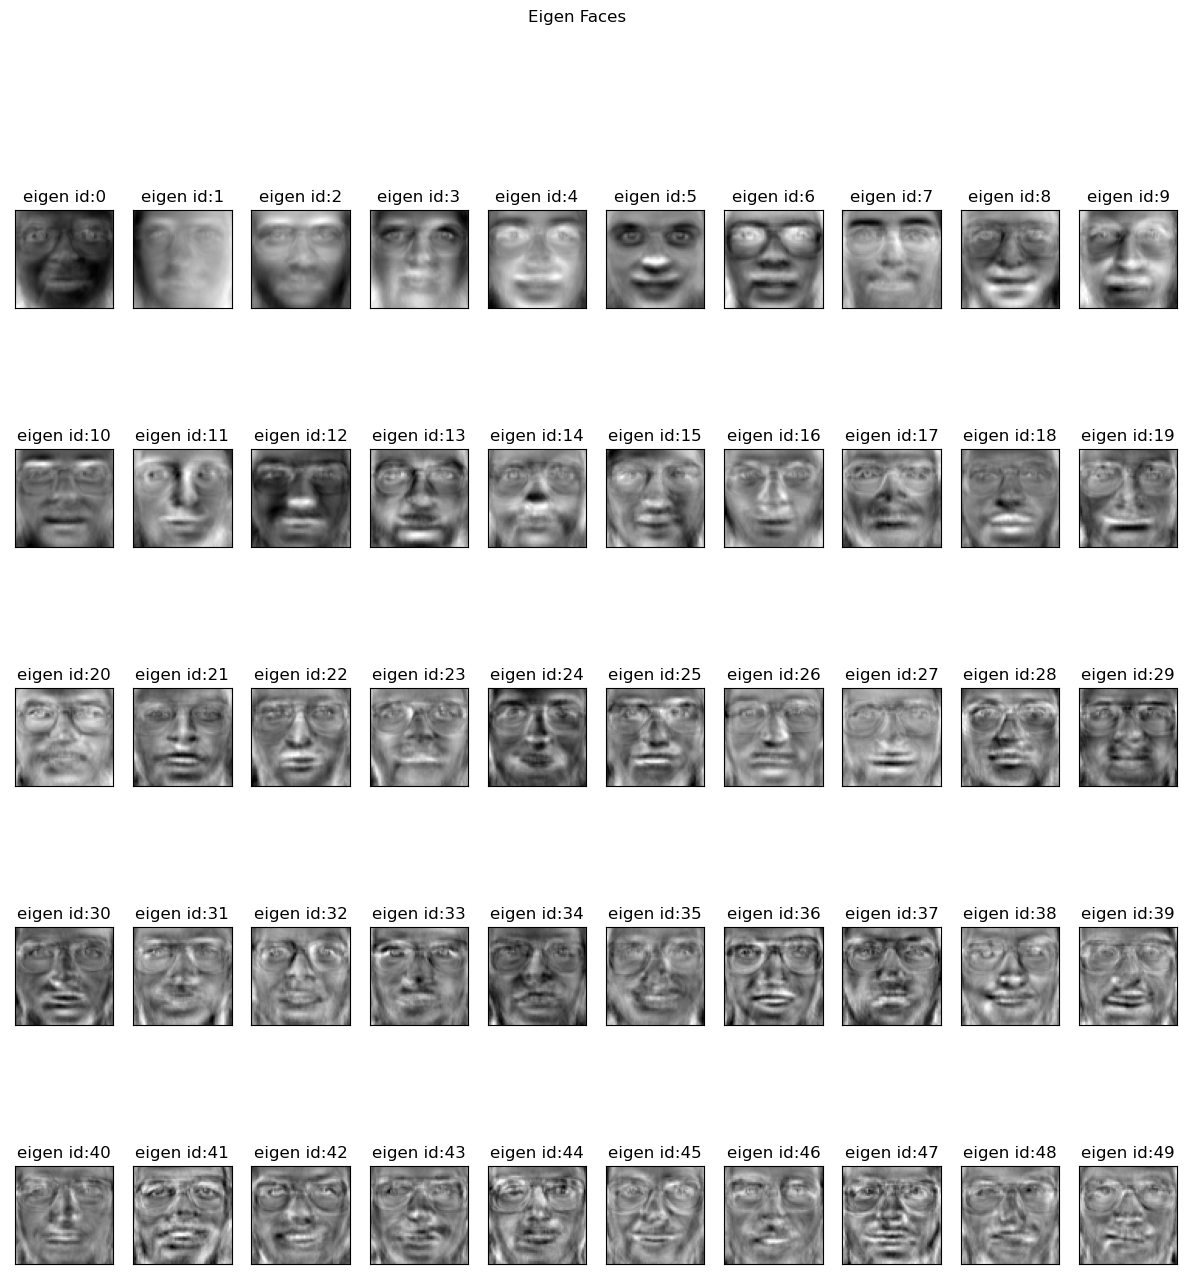
\includegraphics[width=3.8in]{cnn/output.png}
    \caption{Eigen Faces after PCA}
    \label{img:eigen_faces.png}
\end{figure}

\section{Machine Learning Models}

In each implemented machine learning algorithm, we run the algorithm with the base model, with the hyper-parameter selection model, and with K-Fold Cross Validation on the hyper-parameter selection model. For the execution of the described models, we created a function that trains the model passed as an argument and shows graphs, tables, and data in the output, in order to facilitate the analysis of the model.
We also implemented a function that, through the sklearn.model\_selection. GridSearchCV library \cite{grid-search-cV}, performs an exhaustive search on a list of parameters, training a given model with all the parameters, in the end, we return the parameters that gave the best performance, according to the accuracy strategy.

We developed a function that splits the data set into k mixed sets, with training/test indices, using the sklearn.model\_selection.KFold feature \cite{k-fold}. Still, within the function, we evaluate the metrics by cross-validation and record the fit/score times through sklearn.model\_selection.cross\_validate \cite{cross-validate}.

Finally, we create a function that calculates training and testing scores for an estimator with several different values on a specific parameter, these calculations are performed with the sklearn.model\_selection.validation\_curve \cite{validation-curve}. We then graphed the average training scores, and the average test scores, on each specific parameter value.

\subsection{Logistic Regression}
The Logistic Regression \cite{logistic-regression-def} algorithm determines the probability of a binary event (which has only two different results). The Logistic Regression category is supervised learning.

In our problem, we use this algorithm, where the binary results are malignant or benign cancer. We performed the algorithm using the sklearn.linear\_model.LogisticRegression library \cite{logistic-regression}, and with the previously described functions.

\subsection{Gaussian Naive Bayes}
Gaussian Naive Bayes \cite{gnb}is a probabilistic machine learning algorithm that is used for classification tasks. It is based on the Bayes theorem and assumes that the data follows a normal (Gaussian) distribution. The algorithm uses the probability density function of the normal distribution to estimate the probability of a given sample belonging to each class. It then classifies the sample into the class with the highest probability.

\subsection{Support Vector Machine}
SVM \cite{svm-def} is a supervised learning algorithm, which analyzes data for classification and regression observation. Considering a set of training examples, where each example belongs to a category (there are two categories, two results), the SVM algorithm builds a model that classifies new data to a category. This classifier is a non-probabilistic linear binary. Examples are mapped to points in space, with a wide gap between categories. We use sklearn.svm.SVC \cite{svm} to develop this algorithm.

\subsection{k-Nearest Neighbor}
k-NN \cite{knn-def} is a non-parametric, supervised learning algorithm that uses the proximity of points to classify or predict, assuming that similar points are close. We implemented the algorithm using the sklearn.neighbors.KNeighborsClassifier \cite{knn} library.

\subsection{Decision Tree}
Decision Tree \cite{tree-def} is supervised learning, presents a tree structure, the internal nodes are the characteristics of a dataset, the branches are the decision conditions, and the leaf nodes are the results. Graphically represents all possible solutions to a problem. In the development of the algorithm, we used sklearn.tree\_DecisionTreeClassifier \cite{tree}.

\subsection{Linear Discriminante Analysis}
Linear Discriminant Analysis (LDA) \cite{lda} is a supervised machine learning algorithm that is used for classification problems. It is a simple and powerful technique that finds a linear combination of features that separates different classes most effectively. The basic idea behind LDA is to project the data onto a lower-dimensional space where the classes are well-separated. This is achieved by maximizing the ratio of the between-class variance to the within-class variance.

\subsection{CNN}
Convolutional Neural Networks (CNNs) \cite{cnn} are a type of deep learning algorithm that are commonly used in image and video recognition tasks. They are designed to process data with a grid-like topology, such as an image. CNNs consist of several layers, including convolutional layers, pooling layers, and fully connected layers. The convolutional layers apply a set of filters to the input data to learn local features, such as edges and textures. The pooling layers then reduce the spatial dimension of the data while retaining important features. The fully connected layers combine the features learned by the previous layers and make a final prediction. CNNs have been shown to be highly effective in tasks such as image classification, object detection, and facial recognition.

\section{Results}

\subsection{Logistic Regression}

First, we run this algorithm with the base model, with the hyper-parameter selection model, and with K-Fold cross-validation on the hyper-parameter selection model. In Table \ref{tab:tab1} we can see the parameters chosen in the hyper-parameter selection model.

\begin{table}[ht]
    \centering
    \caption{Best parameters in Logistic Regression} 
    \begin{tabular}{||c c c c c||} 
     \hline
     C & class\_weight & max\_iter & penalty & solver \\ [0.5ex] 
     \hline\hline
     0.1 & balanced & 100 & l2 & liblinear \\ 
    \hline
    \end{tabular}
    \label{tab:tab1}
\end{table}

The value selected for parameter C was 0.1. The higher the value of this parameter, the greater the weight on the training data and the lower the weight on the complexity penalty. The smaller the value of this parameter, the smaller the weight in the training data and the greater the weight in the complexity penalty. This parameter is used to handle extreme data. 

The parameter selected in the class\_weight was “balanced”, this strategy implicitly replicates the class with the lowest weight, until there is the same number of samples as the class with the highest weight.

The chosen max\_iter was 100, that is, the maximum number of iterations for the solvers to converge is 100.

The “l2” parameter was selected for the penalty. This parameter imposes the penalty of the square of the magnitude of the coefficients in the model. Thus reducing the coefficients with less contribution, that is, regularization is performed.

The parameter chosen in the solver was “liblinear”, this strategy is advised in small data sets, such as our set. This strategy behaves like a multiclass classified, through the coordinate descent algorithm, ie, separate binary classifiers are trained for all classes.

\subsubsection{Base Model}
The results of the Base model application can be observed in the Figures \ref{fig:conf_LogReg_1} and \ref{fig:conf_LogReg_r_1}. 

\begin{figure}[H]
    \centering
    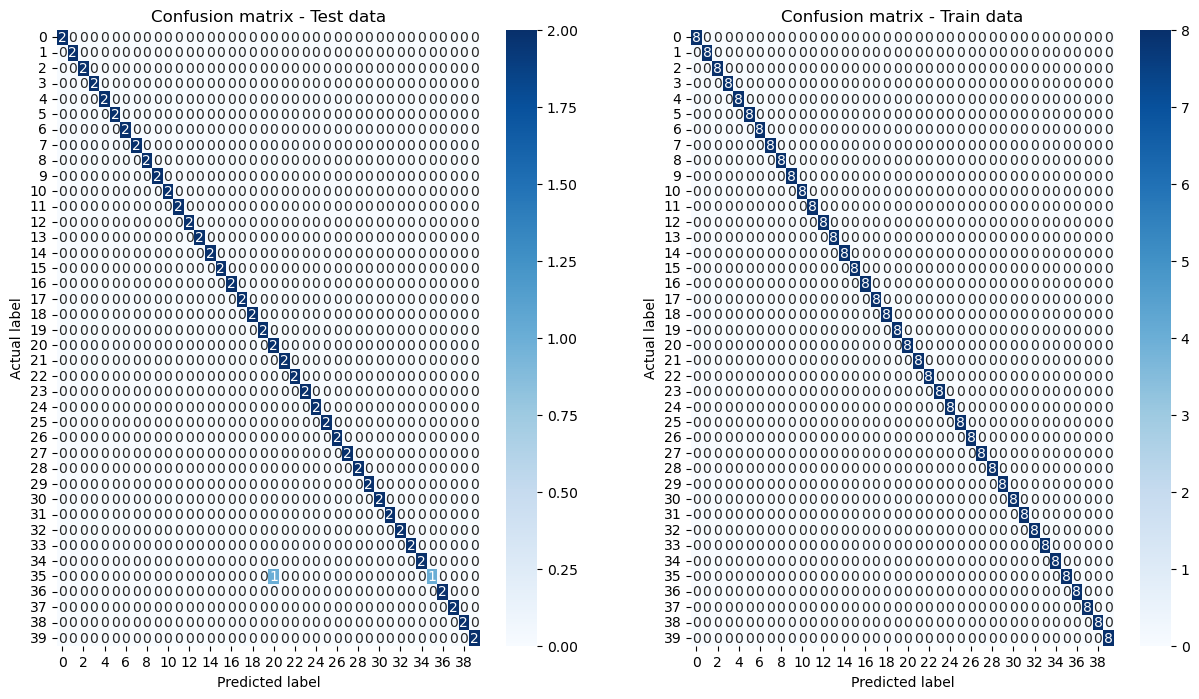
\includegraphics[width=3.8in]{LogReg/logreg_1.png}%
    \caption{Logistic Regression Base Model - Confusion Matrix with Train and Test data}%
    \label{fig:conf_LogReg_1}%
\end{figure}

\begin{figure}[H]
    \centering
    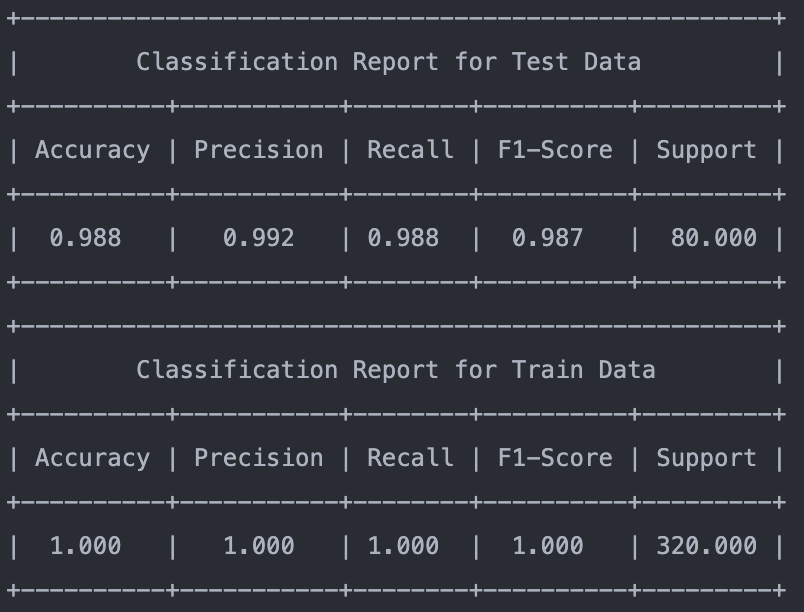
\includegraphics[width=2.8in]{LogReg/logreg_r_1.png}%
    \caption{Logistic Regression Base Model - Table with Test and Train Results for Logistic Regression}%
    \label{fig:conf_LogReg_r_1}%
\end{figure}

\subsubsection{Hyper-Parameter Selection Model}
The results of the Hyper-Parameter Selection Model can be observed in the Figures \ref{fig:conf_LogReg_2} and \ref{fig:conf_LogReg_r_2}. 

\begin{figure}[H]
    \centering
    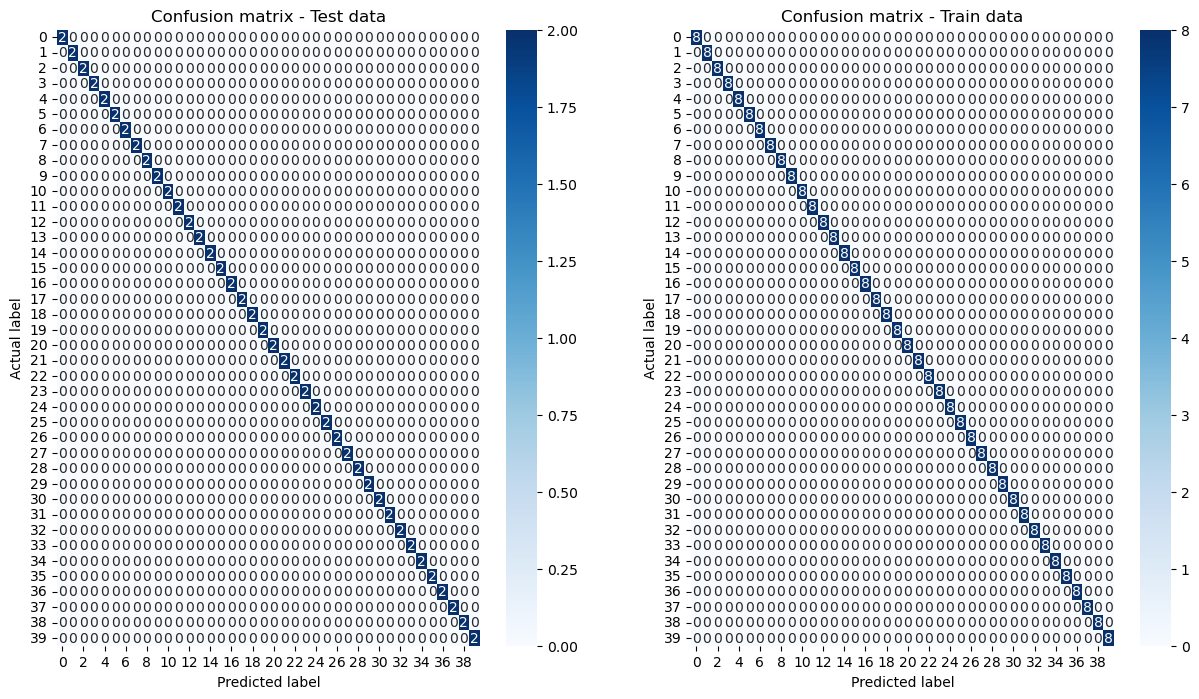
\includegraphics[width=3.8in]{LogReg/logreg_2.png}%
    \caption{Logistic Regression Hyper-Parameter SM - Confusion Matrix with Train and Test data for Logistic Regression}%
    \label{fig:conf_LogReg_2}%
\end{figure}

\begin{figure}[H]
    \centering
    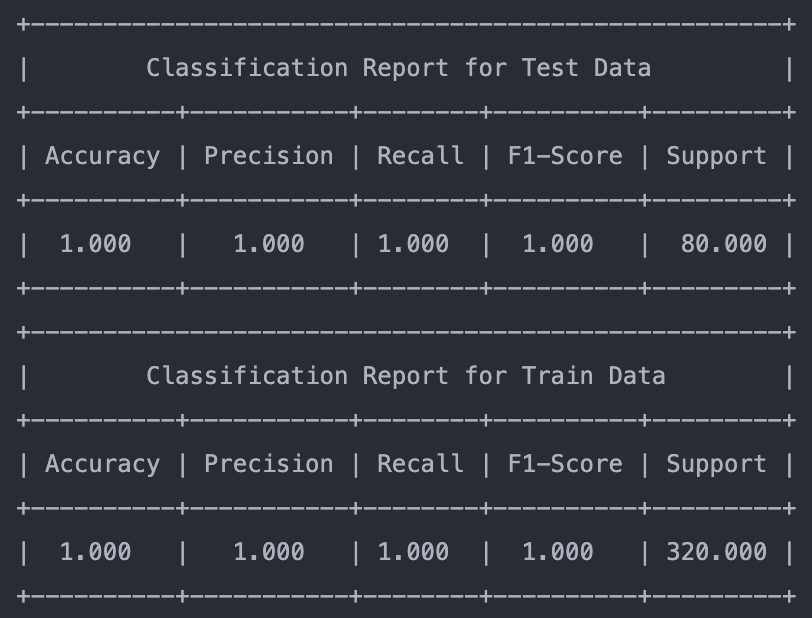
\includegraphics[width=2.8in]{LogReg/logreg_r_2.png}%
    \caption{Logistic Regression Hyper-Parameter SM - Table with Test and Train Results}%
    \label{fig:conf_LogReg_r_2}%
\end{figure}

\subsubsection{K-Fold Cross-Validation Model}
The results of the K-Fold Cross-Validation Model can be observed in the Figures \ref{fig:conf_LogReg_3} and \ref{fig:conf_LogReg_r_3}. 

\begin{figure}[H]
    \centering
    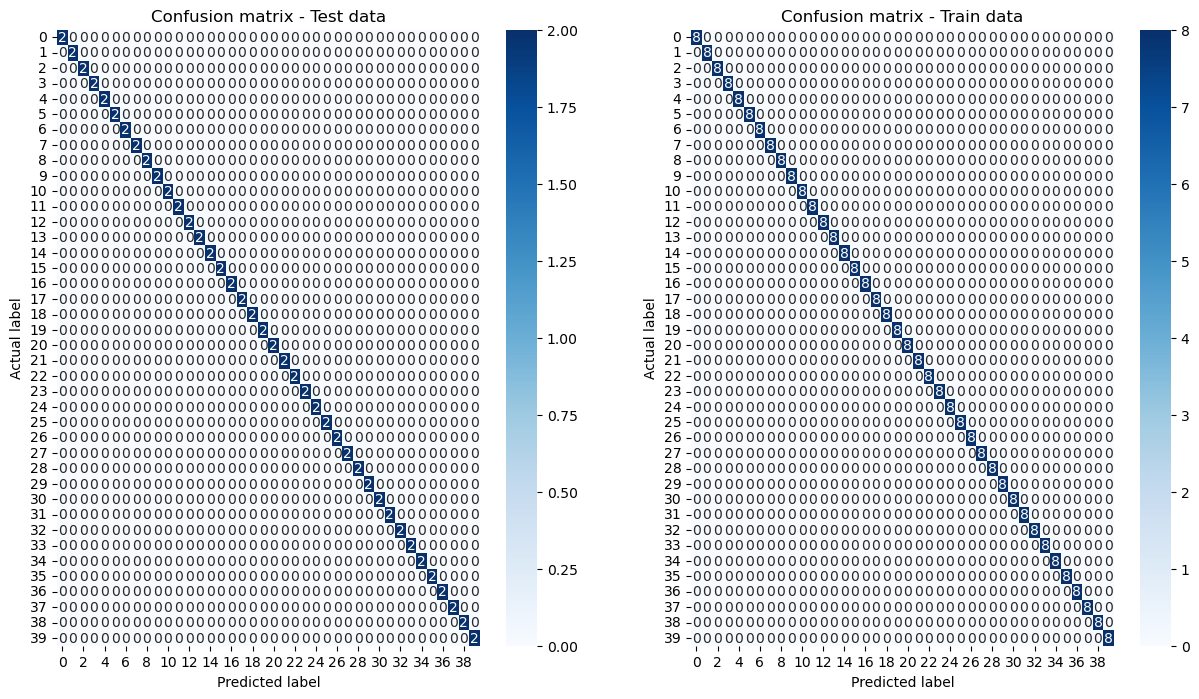
\includegraphics[width=3.8in]{LogReg/logreg_3.png}%
    \caption{Logistic Regression K-Fold CV - Confusion Matrix with Train and Test data}%
    \label{fig:conf_LogReg_3}%
\end{figure}

\begin{figure}[H]
    \centering
    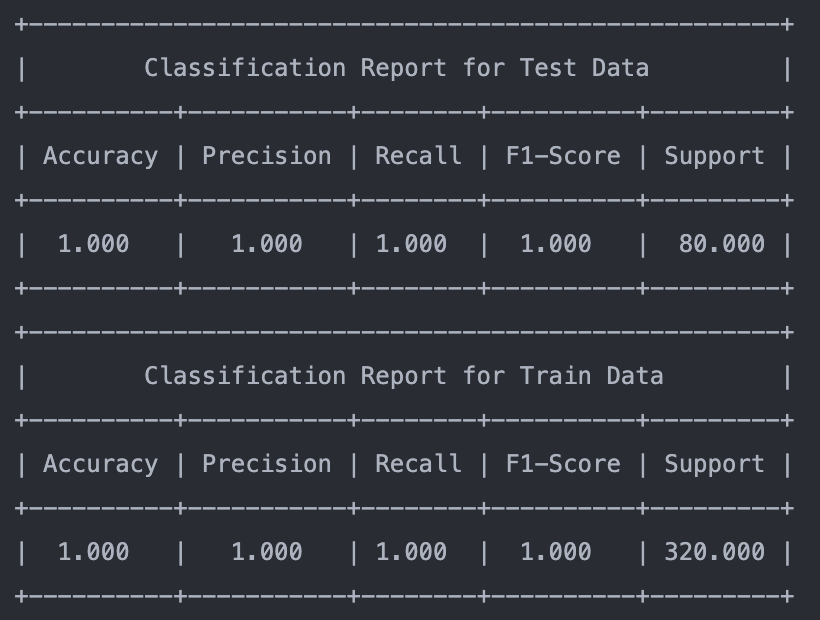
\includegraphics[width=2.8in]{LogReg/logreg_r_3.png}%
    \caption{Logistic Regression K-Fold CV - Table with Test and Train Results}%
    \label{fig:conf_LogReg_r_3}%
\end{figure}

By the figures  \ref{fig:conf_LogReg_r_1}, \ref{fig:conf_LogReg_r_2} and \ref{fig:conf_LogReg_r_3} we can verify that the Accuracy and F1 score of the 3 methods are very identical, with almost no difference in choosing the best method.

\subsection{Gaussian Naive Bayes}

We run this model in three different ways, the base model, the hyper-parameter selection model, and the K-Fold cross-validation with the hyper-parameter selected. The following Table \ref{tab:tab2} shows the parameters chosen by the algorithm.

\begin{table}[H]
    \centering
    \caption{Best parameters in Gaussian Naive Bayes} 
    \begin{tabular}{||c c c c||} 
     \hline
     activation & alpha & hidden\_layer\_sizes & learning\_rate \\[0.5ex] 
     \hline\hline
     relu & 1 & (12, 12) & constant \\ 
    \hline
    \end{tabular}
    \begin{tabular}{||c c c||}
    \hline
    var_smoothing & var_smoothing \\ [0.5ex] 
    \hline\hline
     0.533669923120631 & 0.533669923120631 \\ 
    \hline
    \end{tabular}
    \label{tab:tab2}
\end{table}
\subsubsection{Base Model}
The results of the Base model application can be observed in the Figures \ref{fig:conf_gnb_1} and \ref{fig:conf_gnb_r_1}. 

\begin{figure}[H]
    \centering
    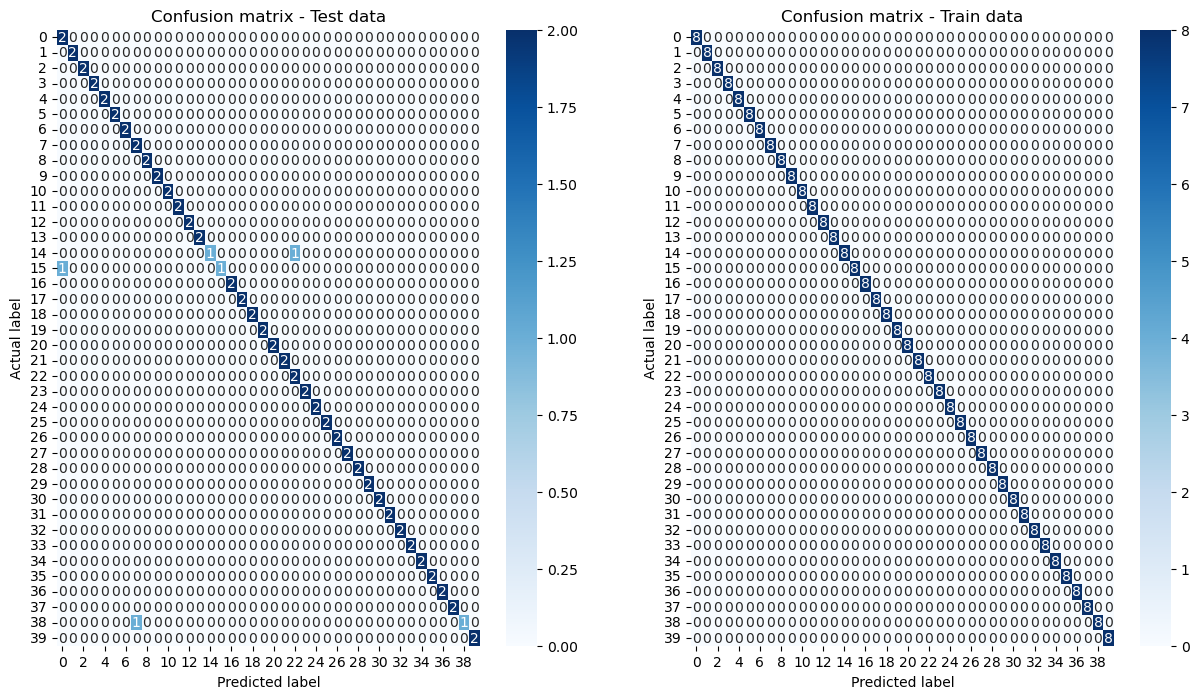
\includegraphics[width=3.8in]{GNB/1.png}%
    \caption{GNB Base Model - Confusion Matrix with Train and Test data}%
    \label{fig:conf_gnb_1}%
\end{figure}

\begin{figure}[H]
    \centering
    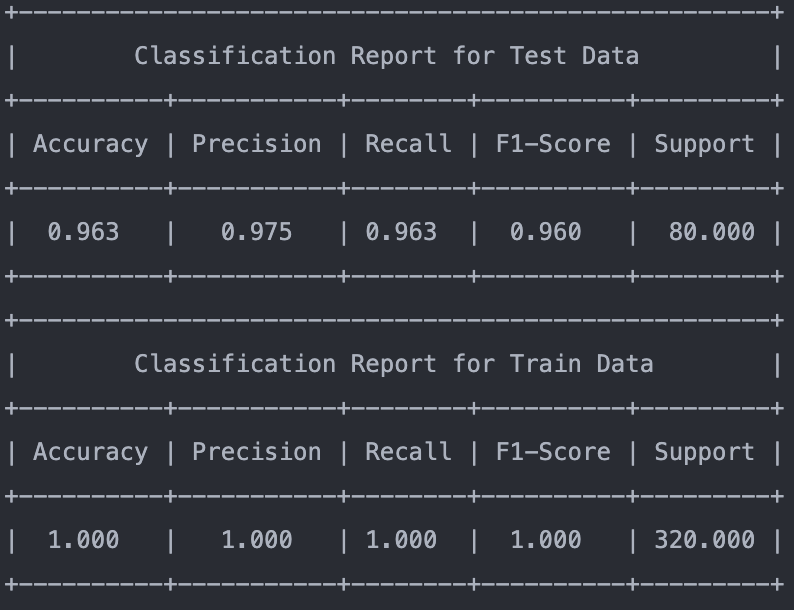
\includegraphics[width=2.8in]{GNB/r_1.png}%
    \caption{GNB Base Model - Table with Test and Train Results}%
    \label{fig:conf_gnb_r_1}%
\end{figure}

\subsubsection{Hyper-Parameter Selection Model}
The results of the Hyper-Parameter Selection Model can be observed in the Figures \ref{fig:conf_gnb_2} and \ref{fig:conf_gnb_r_2}. 

\begin{figure}[H]
    \centering
    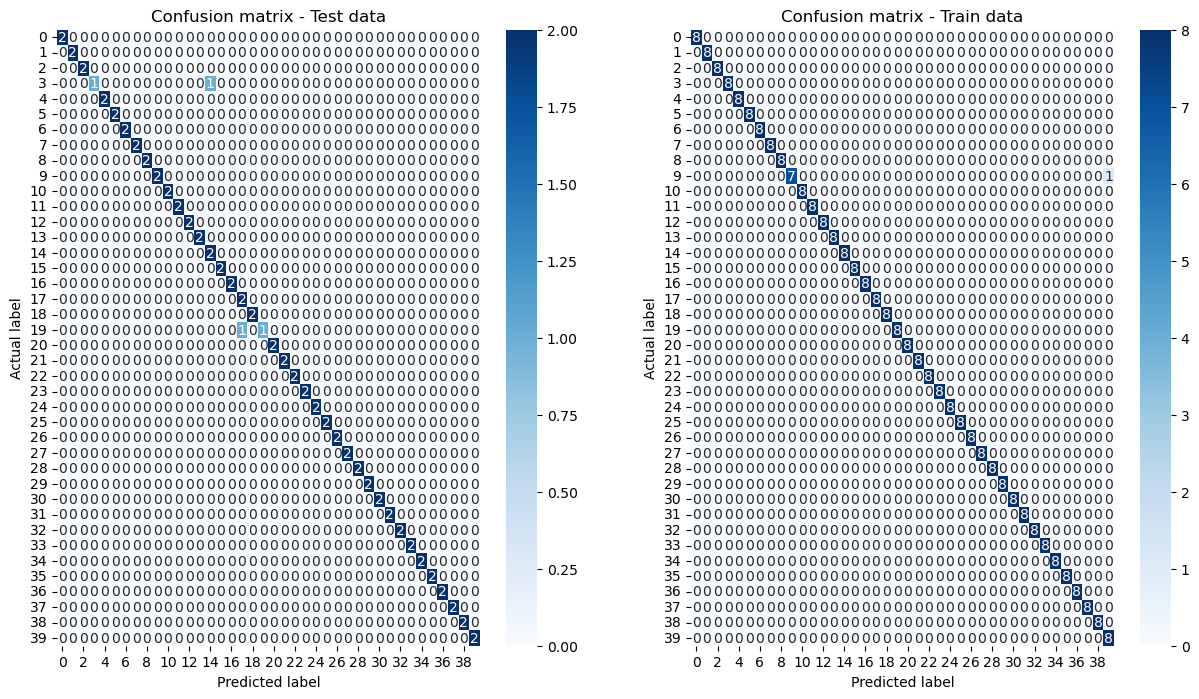
\includegraphics[width=3.8in]{GNB/2.png}%
    \caption{GNB Hyper-Parameter Selection Model - Confusion Matrix with Train and Test data}%
    \label{fig:conf_gnb_2}%
\end{figure}

\begin{figure}[H]
    \centering
    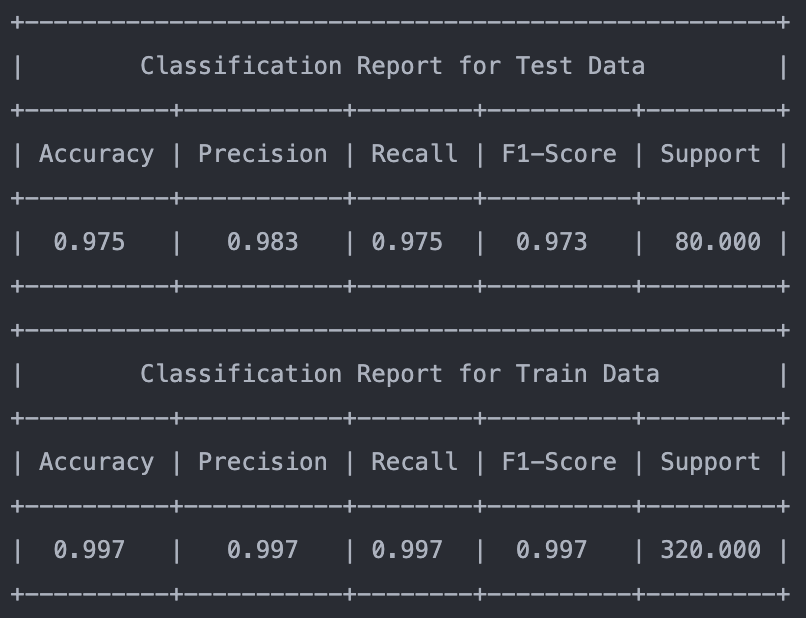
\includegraphics[width=2.8in]{GNB/r_2.png}%
    \caption{GNB Hyper-Parameter Selection Model - Table with Test and Train Results}%
    \label{fig:conf_gnb_r_2}%
\end{figure}

\subsubsection{K-Fold Cross-Validation Model}
The results of the K-Fold Cross-Validation Model can be observed in the Figures \ref{fig:conf_gnb_3} and \ref{fig:conf_gnb_r_3}. 

\begin{figure}[H]
    \centering
    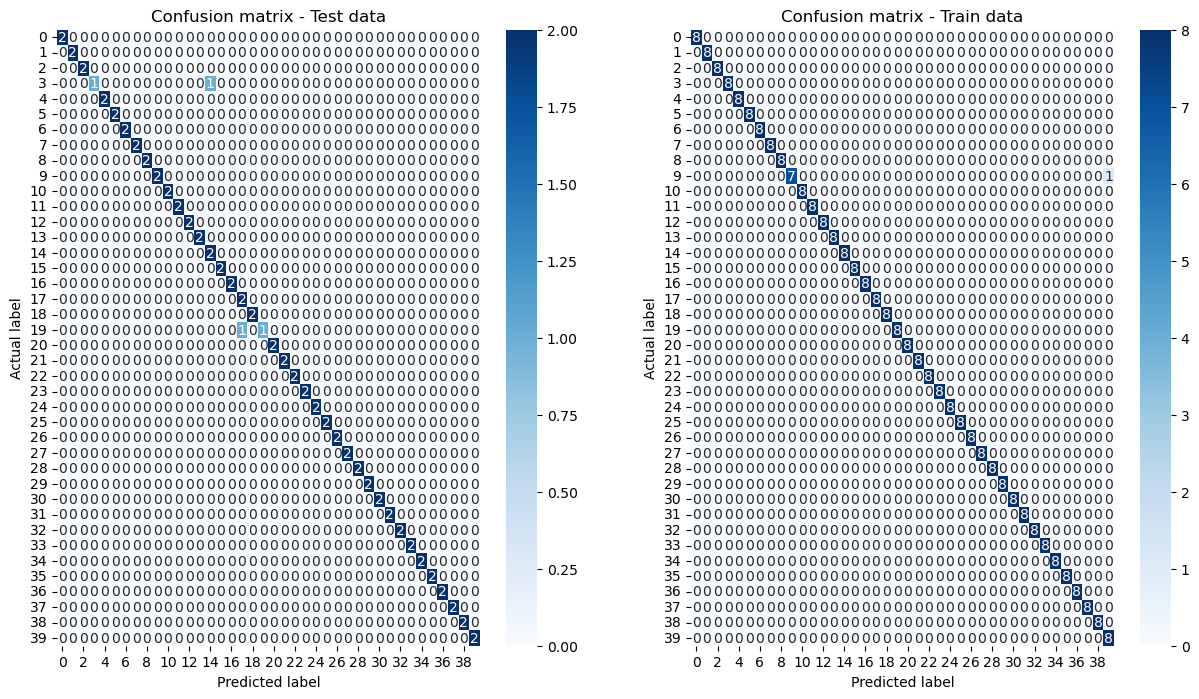
\includegraphics[width=3.8in]{GNB/3.png}%
    \caption{GNB K-Fold CV - Confusion Matrix with Test and Train data}%
    \label{fig:conf_gnb_3}%
\end{figure}

\begin{figure}[H]
    \centering
    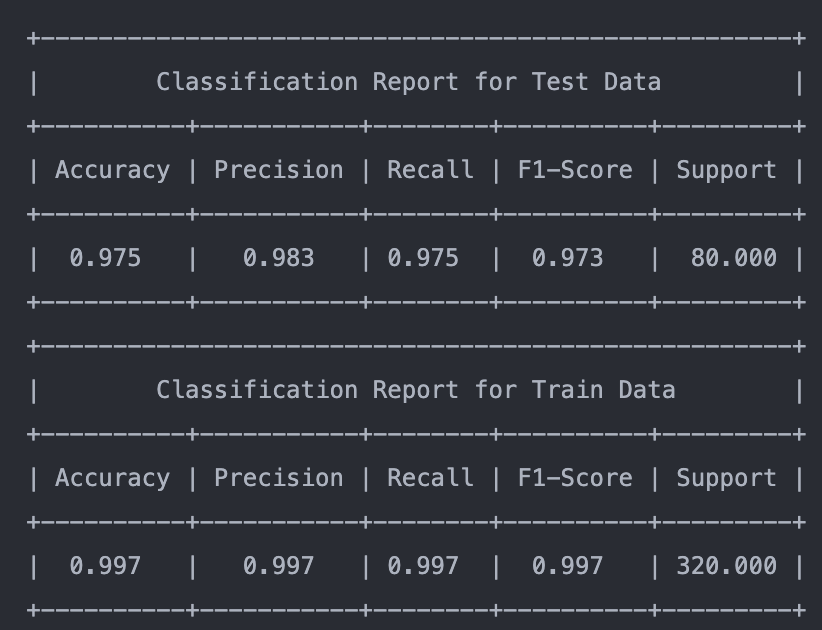
\includegraphics[width=2.8in]{GNB/r_3.png}%
    \caption{GNB K-Fold CV - Table with Test and Train Results}%
    \label{fig:conf_gnb_r_3}%
\end{figure}


%%%%%%%%%%%%%%%%%%%%%%%%%%%%%%%%%%%%SVC%%%%%%%%%%%%%%%%%%%%%%%%%%%%%%%%%%%

\subsection{Support Vector Machine}

We run this model in three different ways, the base model, the hyper-parameter selection model, and the K-Fold cross-validation with the hyper-parameter selected. The following Table \ref{tab:tab-svc} shows the parameters chosen by the algorithm.

\begin{table}[ht!]
    \centering
    \caption{Best parameters in SVM} 
    \begin{tabular}{||c c c c||} 
     \hline
     C & class\_weight & gamma & kernel \\ [0.5ex] 
     \hline\hline
     10 & balanced & 0.01 & rbf \\ 
    \hline
    \end{tabular}
    \label{tab:tab-svc}
\end{table}
\subsubsection{Base Model}
The results of the Base model application can be observed in the Figures \ref{fig:conf_svm_1} and \ref{fig:conf_svm_r_1}. 

\begin{figure}[H]
    \centering
    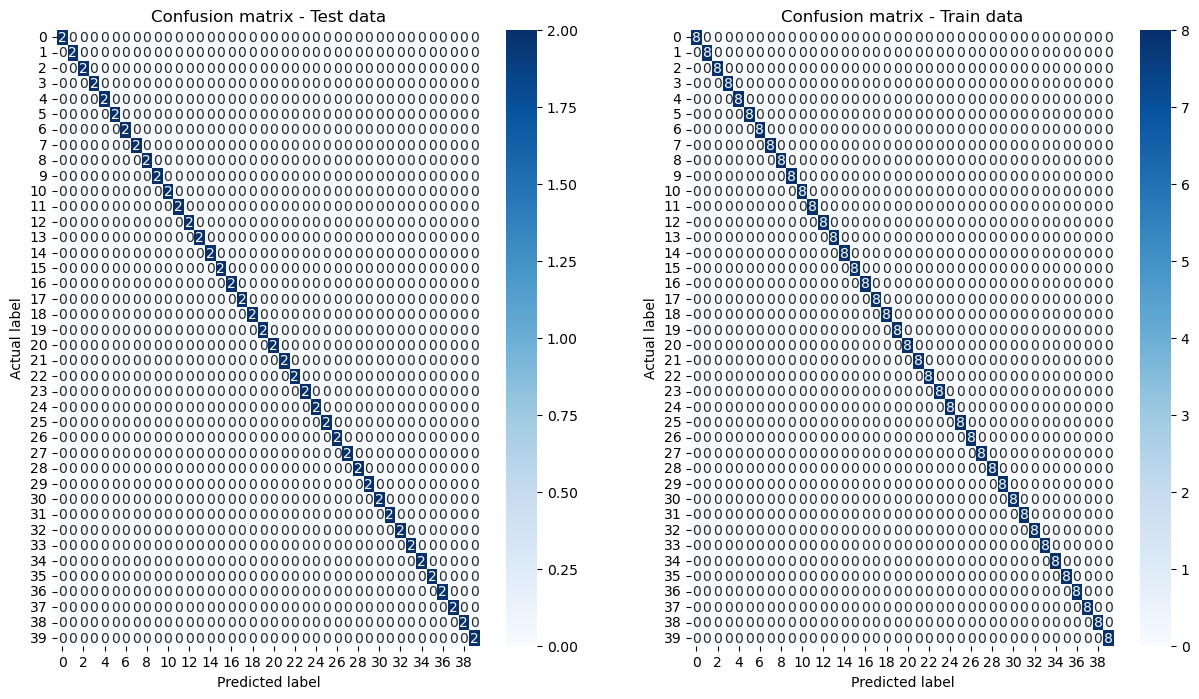
\includegraphics[width=3.8in]{SVC/1.png}%
    \caption{SVM Base Model - Confusion Matrix with Train and Test data}%
    \label{fig:conf_svm_1}%
\end{figure}

\begin{figure}[H]
    \centering
    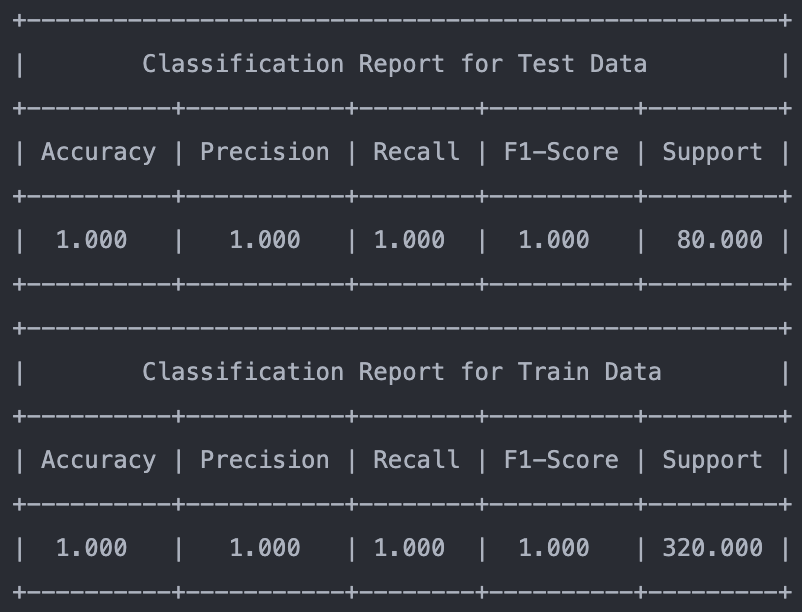
\includegraphics[width=2.8in]{SVC/r_1.png}%
    \caption{SVM Base Model - Table with Test and Train Results}%
    \label{fig:conf_svm_r_1}%
\end{figure}

\subsubsection{Hyper-Parameter Selection Model}
The results of the Hyper-Parameter Selection Model can be observed in the Figures \ref{fig:conf_svm_2} and \ref{fig:conf_svm_r_2}.

\begin{figure}[H]
    \centering
    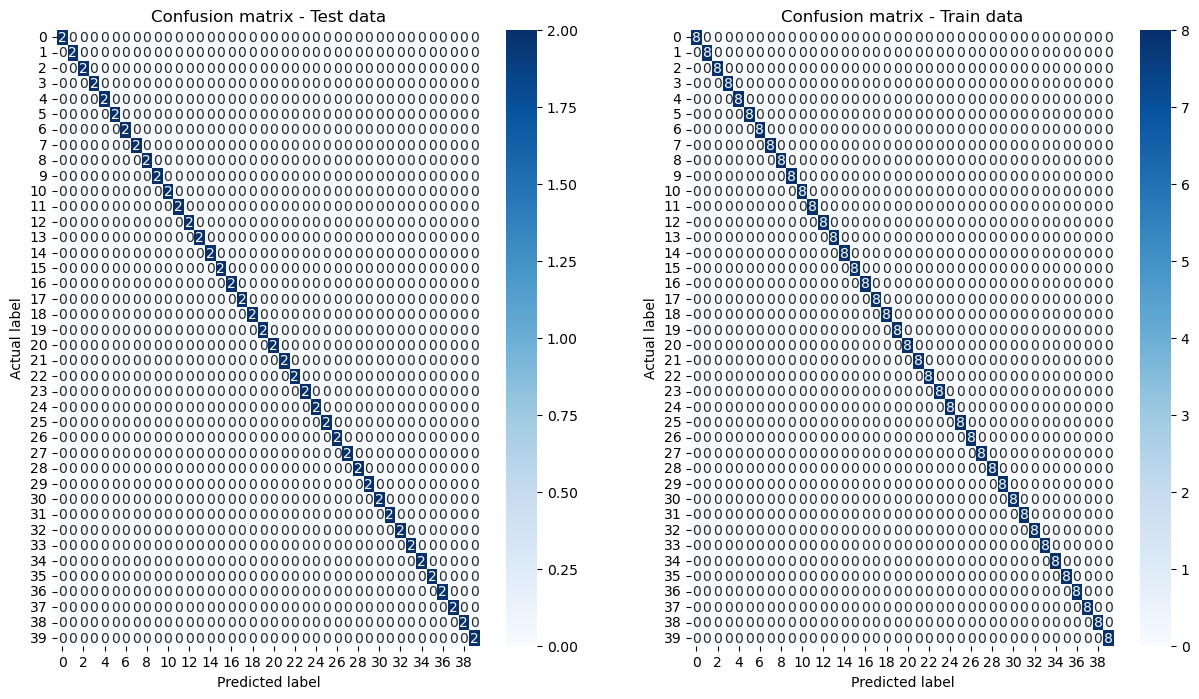
\includegraphics[width=3.8in]{SVC/2.png}%
    \caption{SVM Hyper-Parameter SM - Confusion Matrix with Train and Test data}%
    \label{fig:conf_svm_2}%
\end{figure}

\begin{figure}[H]
    \centering
    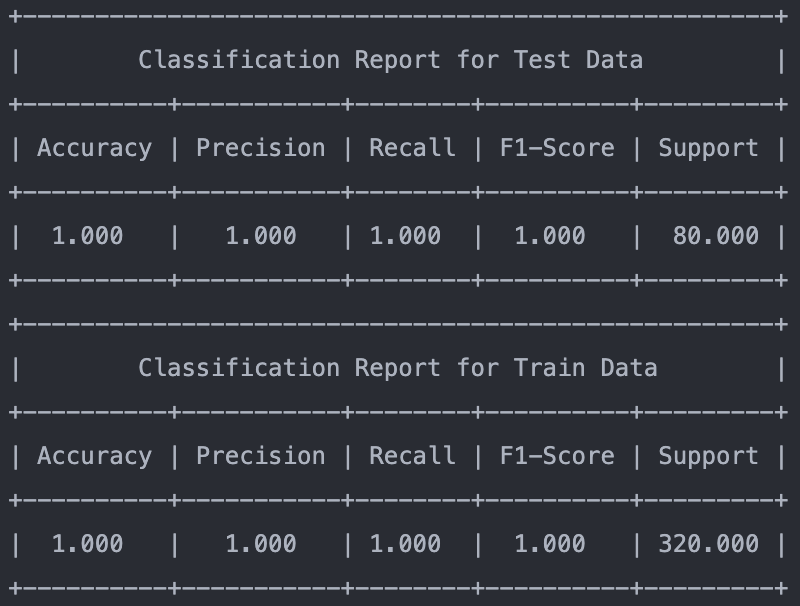
\includegraphics[width=2.8in]{SVC/r_2.png}%
    \caption{SVM Hyper-Parameter SM - Table with Test and Train Results}%
    \label{fig:conf_svm_r_2}%
\end{figure}

\subsubsection{K-Fold Cross-Validation Model}
The results of the K-Fold Cross-Validation Model can be observed in the Figures \ref{fig:conf_svm_3} and \ref{fig:conf_svm_r_3}. 

\begin{figure}[H]
    \centering
    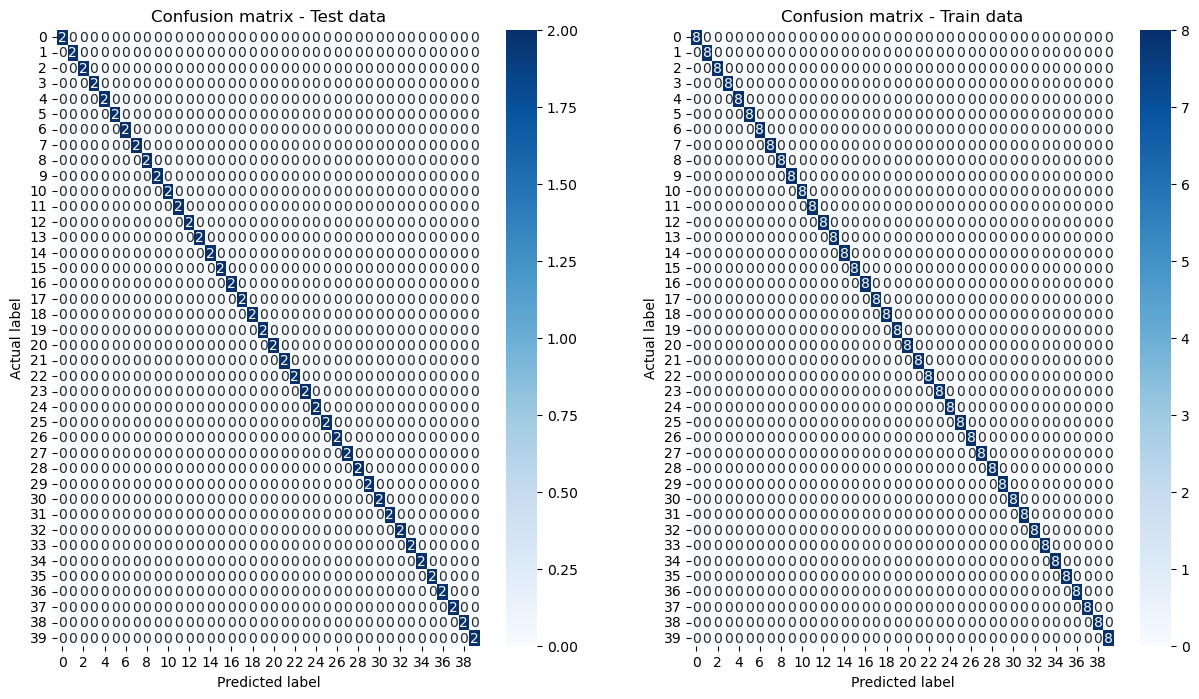
\includegraphics[width=3.8in]{SVC/3.png}%
    \caption{SVM K-Fold CV - Confusion Matrix with Train and Test data}%
    \label{fig:conf_svm_3}%
\end{figure}

\begin{figure}[H]
    \centering
    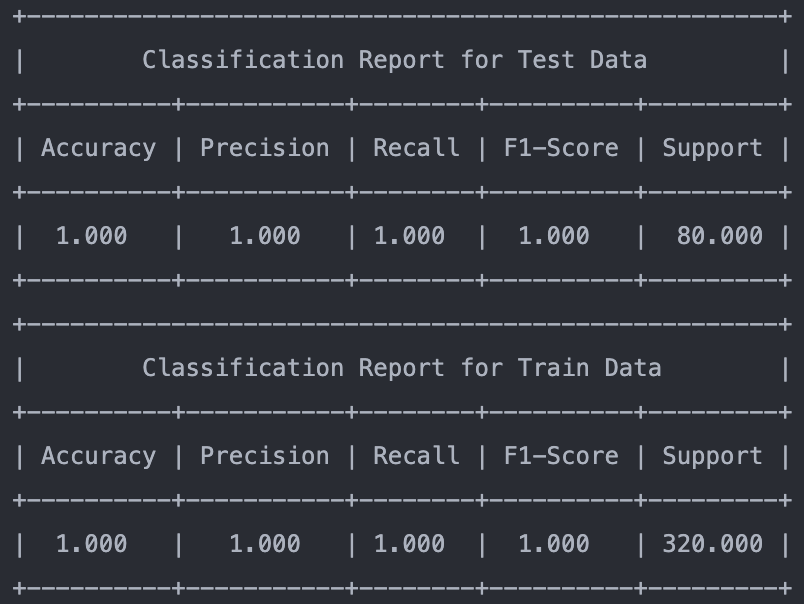
\includegraphics[width=2.8in]{SVC/r_3.png}%
    \caption{SVM K-Fold CV - Table with Test and Train Results}%
    \label{fig:conf_svm_r_3}%
\end{figure}

%%%%%%%%%%%%%%%%%%%%%%%%%%%%%%%%%%%%%%%%%k-Nearest Neighbor%%%%%%%%%%%%%%%%%%%%%%%%%%%%%%%%%%%%%%%%%%%%
\subsection{k-Nearest Neighbor}

We run this model in three different ways, the base model, the hyper-parameter selection model, and the K-Fold Cross Validation with the hyper-parameter selected. The following Table \ref{tab:tab5} shows the parameters chosen by the algorithm.

\begin{table}[H]
    \centering
    \begin{tabular}{||c c c c||} 
     \hline
     algorithm & n_neighbors & weights \\[0.5ex] 
     \hline\hline
     auto & 3 & distance \\ 
    \hline
    \end{tabular}
    \caption{Best parameters in K-Nearest Neighbor} 
    \label{tab:tab5}
\end{table}
\subsubsection{Base Model}
The results of the Base model application can be observed in the Figures \ref{fig:conf_knn_1} and \ref{fig:conf_knn_r_1}. 

\begin{figure}[H]
    \centering
    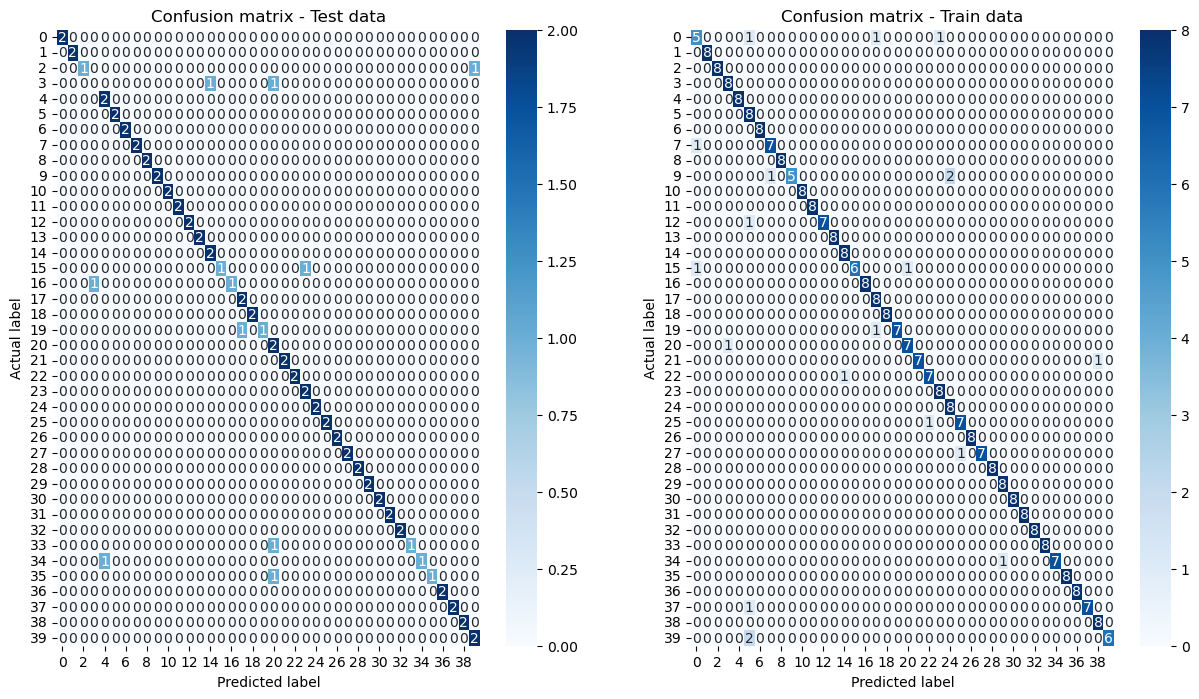
\includegraphics[width=3.8in]{k-NN/1.png}%
    \caption{kNN Base Model - Confusion Matrix with Train and Test data}%
    \label{fig:conf_knn_1}%
\end{figure}

\begin{figure}[H]
    \centering
    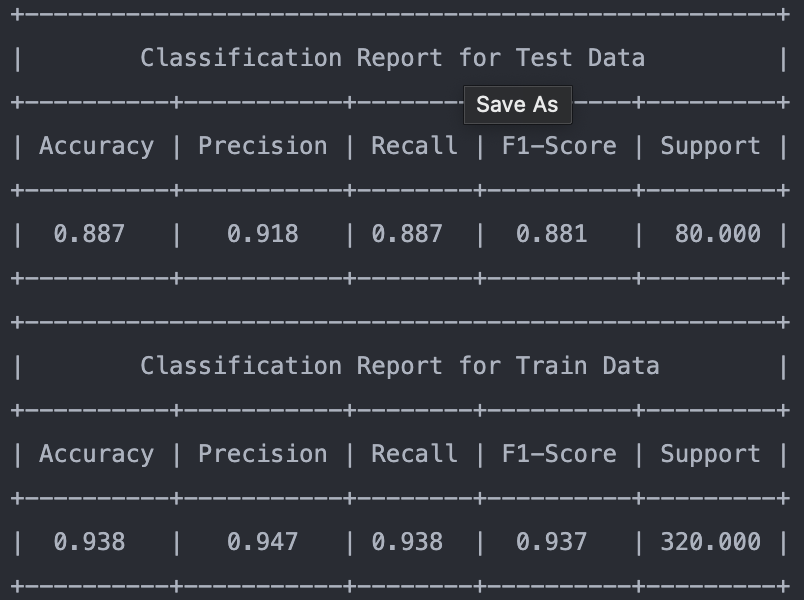
\includegraphics[width=2.8in]{k-NN/r_1.png}%
    \caption{kNN Base Model - Table with Test and Train Results}%
    \label{fig:conf_knn_r_1}%
\end{figure}

\subsubsection{Hyper-Parameter Selection Model}
The results of the Hyper-Parameter Selection Model can be observed in the Figures \ref{fig:conf_knn_2} and \ref{fig:conf_knn_r_2}.

\begin{figure}[H]
    \centering
    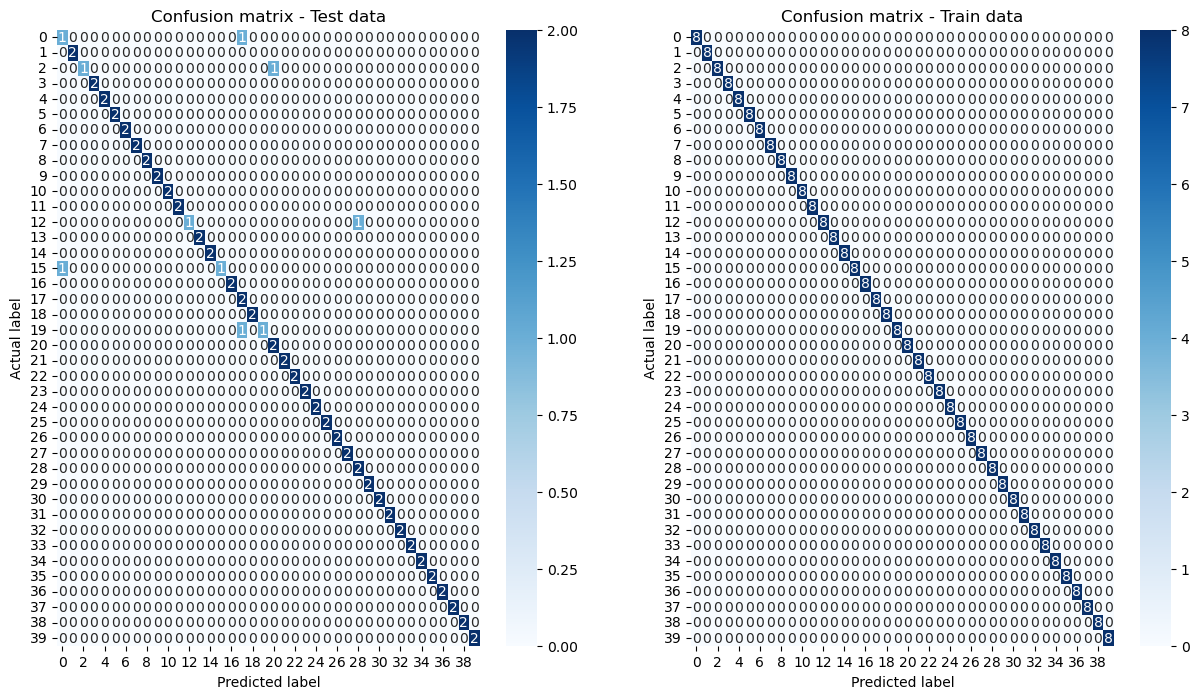
\includegraphics[width=3.8in]{k-NN/2.png}%
    \caption{kNN Hyper-Parameter SM - Confusion Matrix with Train and Test data}%
    \label{fig:conf_knn_2}%
\end{figure}

\begin{figure}[H]
    \centering
    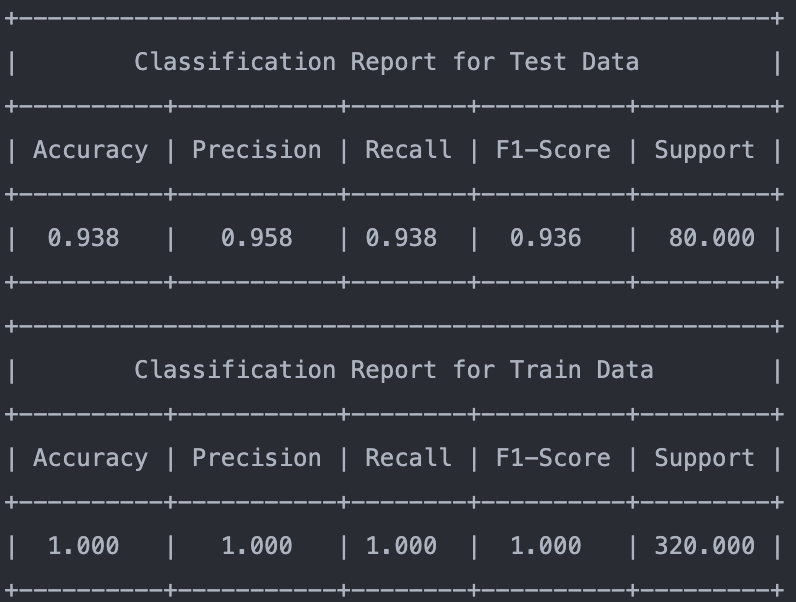
\includegraphics[width=2.8in]{k-NN/r_2.png}%
    \caption{kNN Hyper-Parameter SM - Table with Test and Train Results}%
    \label{fig:conf_knn_r_2}%
\end{figure}

\subsubsection{K-Fold Cross-Validation Model}
The results of the K-Fold Cross-Validation Model can be observed in the Figures \ref{fig:conf_knn_3} and \ref{fig:conf_knn_r_3}.

\begin{figure}[H]
    \centering
    \includegraphics[width=3.8in]{k-NN/3.png}%
    \caption{kNN K-Fold CV - Confusion Matrix with Train and Test data}%
    \label{fig:conf_knn_3}%
\end{figure}

\begin{figure}[H]
    \centering
    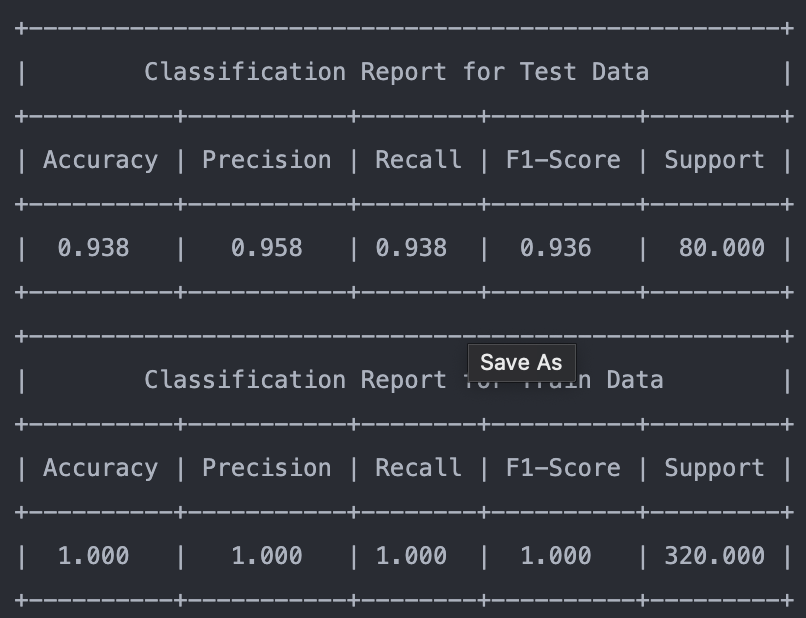
\includegraphics[width=2.8in]{k-NN/r_3.png}%
    \caption{kNN K-Fold CV - Table with Test and Train Results}%
    \label{fig:conf_knn_r_3}%
\end{figure}


%%%%%%%%%%%%%%%%%%%%%%%%%%%%%%%%%%%%%%%%%Decision Tree%%%%%%%%%%%%%%%%%%%%%%%%%%%%
\subsection{Decision Tree}
We run this model in three different ways, the base model, the hyper-parameter selection model, and the K-Fold cross-validation with the hyper-parameter selected. The following Table \ref{tab:tab6} shows the parameters chosen by the algorithm.

\begin{table}[H]
    \centering
    \begin{tabular}{||c c c c c||} 
     \hline
     criterion & max\_depth & min\_samples\_leaf & min\_samples\_split & splitter \\[0.5ex] 
     \hline\hline
     entropy & 8 & 1 & 7 & best \\ 
    \hline
    \end{tabular}
    \caption{Best parameters in Decision Tree} 
    \label{tab:tab6}
\end{table}
\subsubsection{Base Model}
The results of the Base model application can be observed in the Figures \ref{fig:conf_dt_1} and \ref{fig:conf_dt_r_1}. 

\begin{figure}[H]
    \centering
    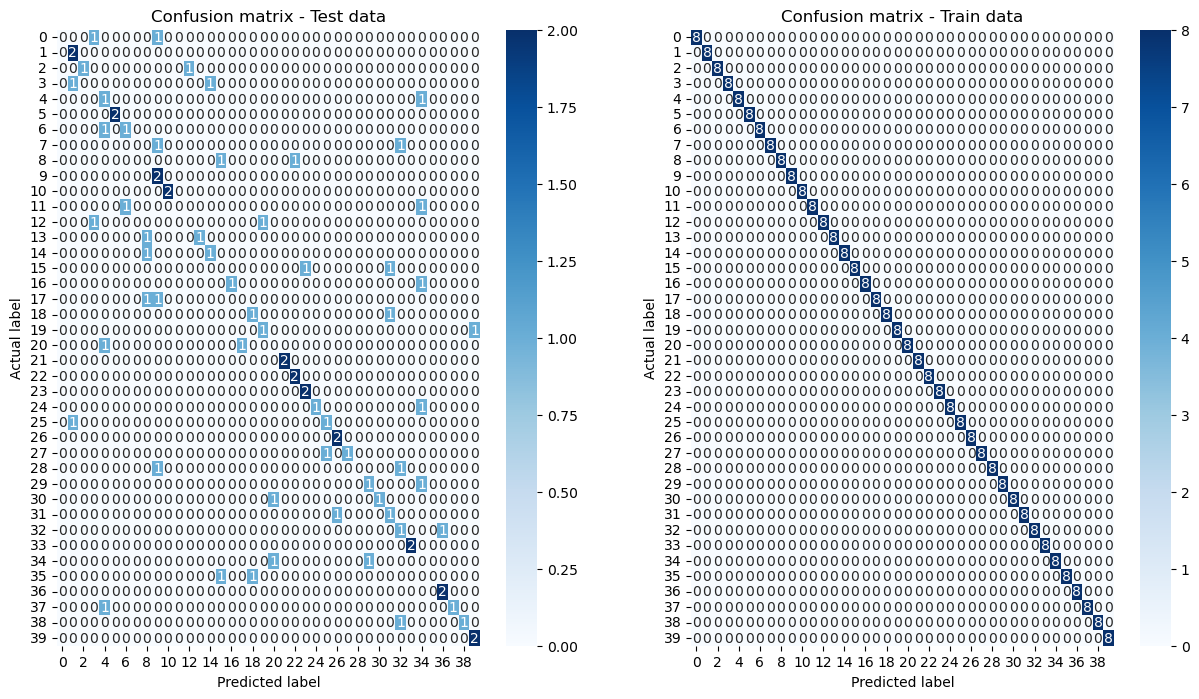
\includegraphics[width=3.8in]{DT/1.png}%
    \caption{Decision Tree Base Model - Confusion Matrix with Train and Test data}%
    \label{fig:conf_dt_1}%
\end{figure}

\begin{figure}[H]
    \centering
    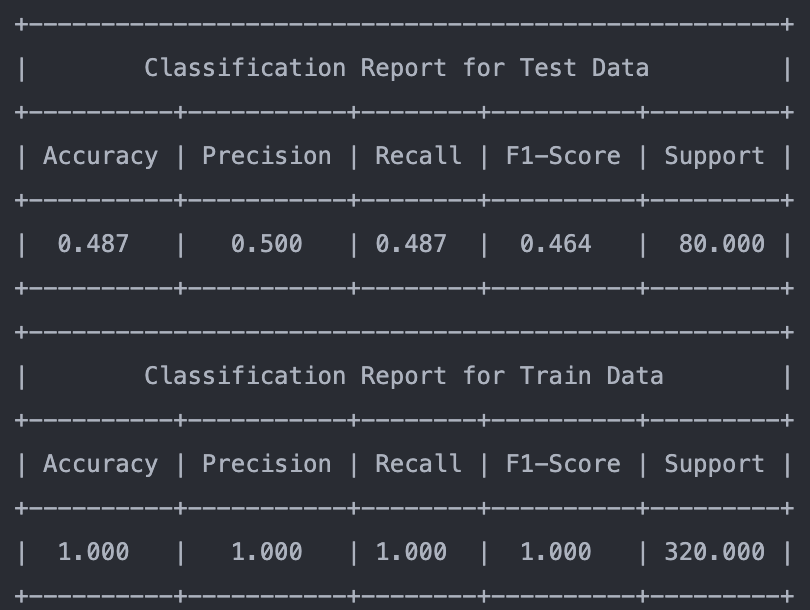
\includegraphics[width=2.8in]{DT/Screenshot 2023-01-21 at 01.15.28.png}%
    \caption{Decision Tree Base Model - Table with Test and Train Results}%
    \label{fig:conf_dt_r_1}%
\end{figure}

\subsubsection{Hyper-Parameter Selection Model}
The results of the Hyper-Parameter Selection Model can be observed in the Figures \ref{fig:conf_dt_2} and \ref{fig:conf_dt_r_2}.

\begin{figure}[H]
    \centering
    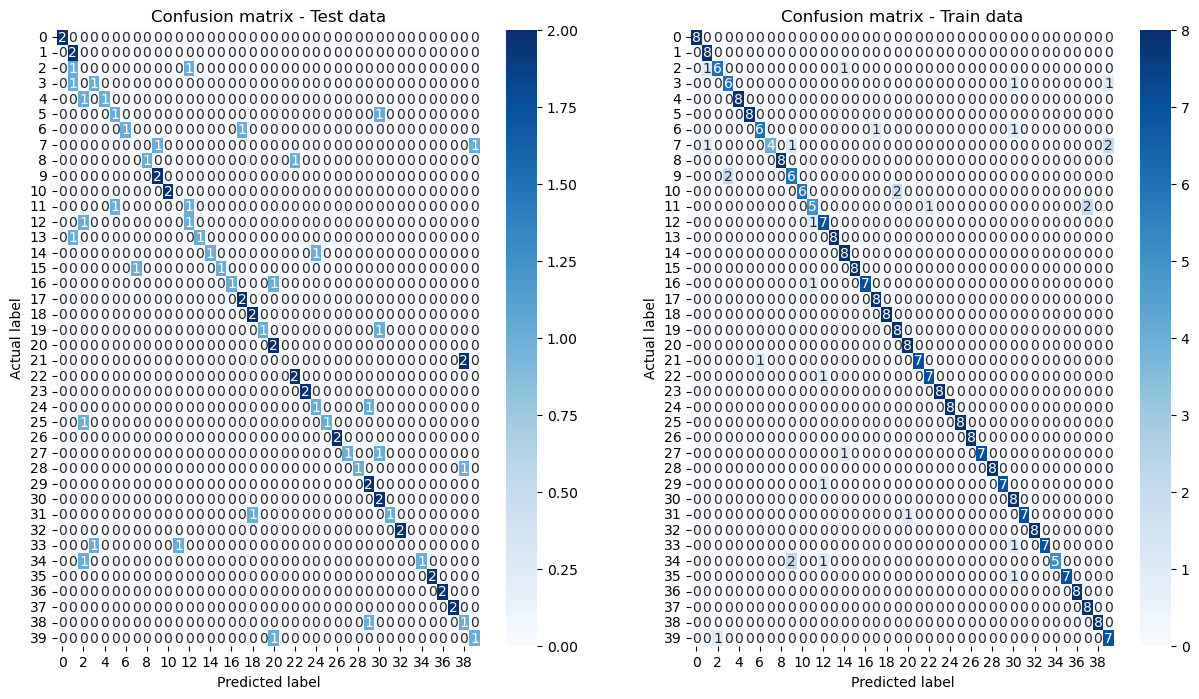
\includegraphics[width=3.8in]{DT/2.png}%
    \caption{Decision Tree Hyper-Parameter SM - Confusion Matrix with Train and Test data}%
    \label{fig:conf_dt_2}%
\end{figure}

\begin{figure}[H]
    \centering
    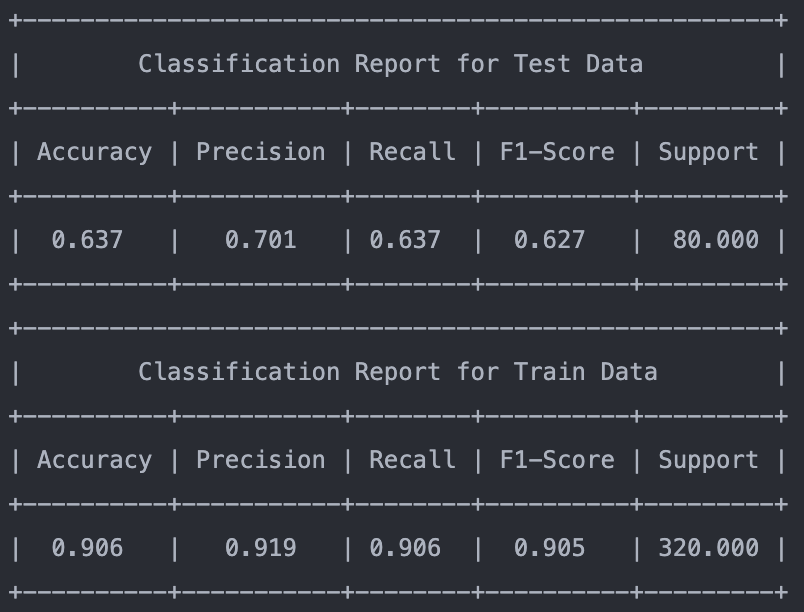
\includegraphics[width=2.8in]{DT/Screenshot 2023-01-21 at 01.15.37.png}%
    \caption{Decision Tree Hyper-Parameter SM - Table with Test and Train Results}%
    \label{fig:conf_dt_r_2}%
\end{figure}

\subsubsection{K-Fold Cross-Validation Model}
The results of the K-Fold Cross-Validation Model can be observed in the Figures \ref{fig:conf_dt_3} and \ref{fig:conf_dt_r_3}.

\begin{figure}[H]
    \centering
    \includegraphics[width=3.8in]{DT/3.png}%
    \caption{Decision Tree K-Fold CV - Confusion Matrix with Train and Test data}%
    \label{fig:conf_dt_3}%
\end{figure}

\begin{figure}[H]
    \centering
    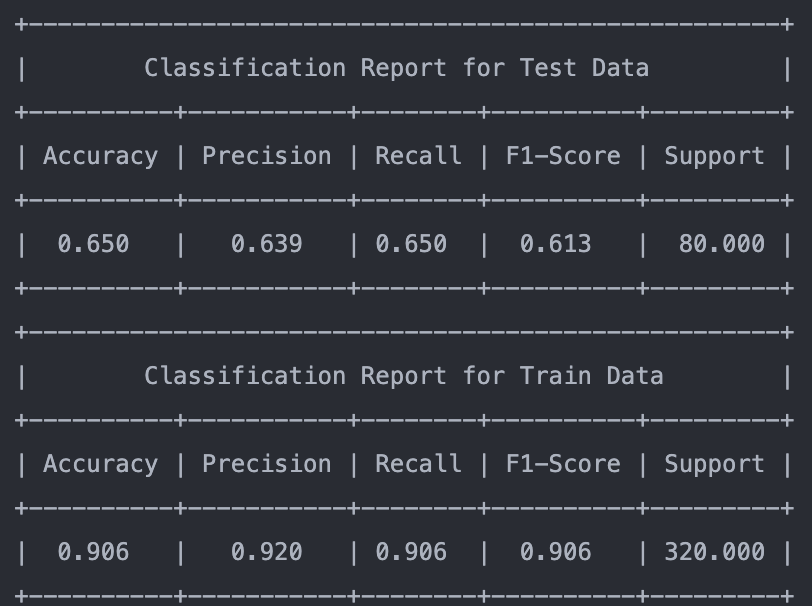
\includegraphics[width=2.8in]{DT/Screenshot 2023-01-21 at 01.15.42.png}%
    \caption{Decision Tree K-Fold CV - Table with Test and Train Results}%
    \label{fig:conf_dt_r_3}%
\end{figure}

\subsection{CNN}
The results of the CNN can be observed in the Figure \ref{fig:results_cnn}.

\begin{figure}
    \centering
    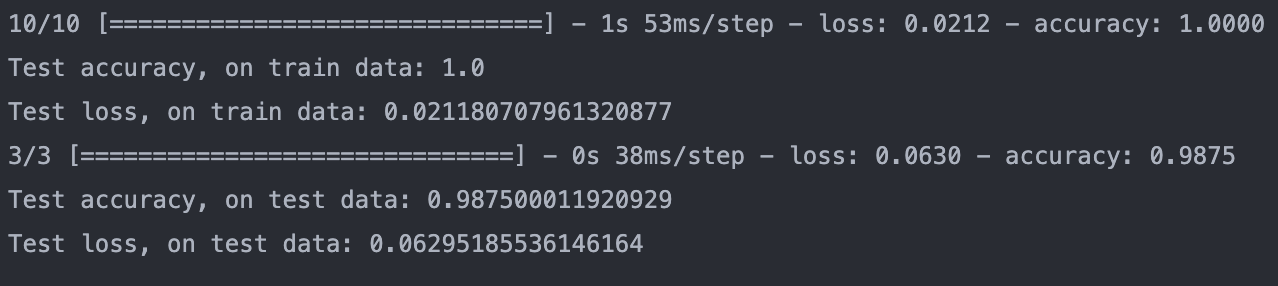
\includegraphics[width=3in]{cnn/Screenshot 2023-01-21 at 02.04.01.png}
    \caption{Results}
    \label{fig:results_cnn}
\end{figure}

This model was built with the parameters shown in Figure \ref{fig:cnn_model}.
\begin{figure}
    \centering
    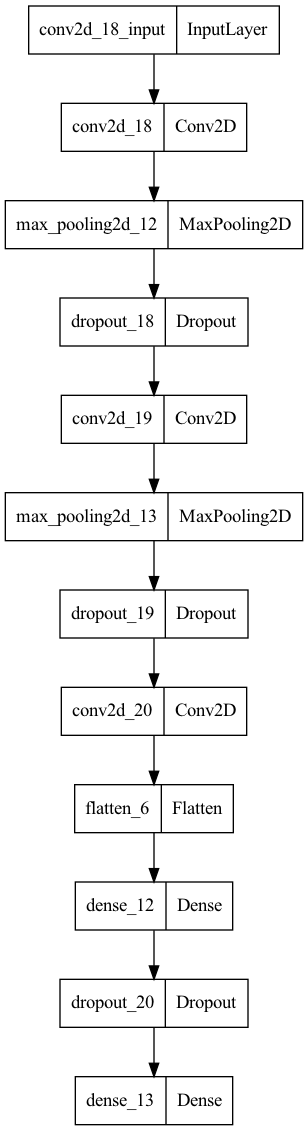
\includegraphics[width=1in]{cnn/2.png}
    \caption{Model}
    \label{fig:cnn_model}
\end{figure}



In the Figure \ref{fig:accuracy_vs_epoch} we can see the evolution of the accuracy through the number of epochs.

\begin{figure}
    \centering
    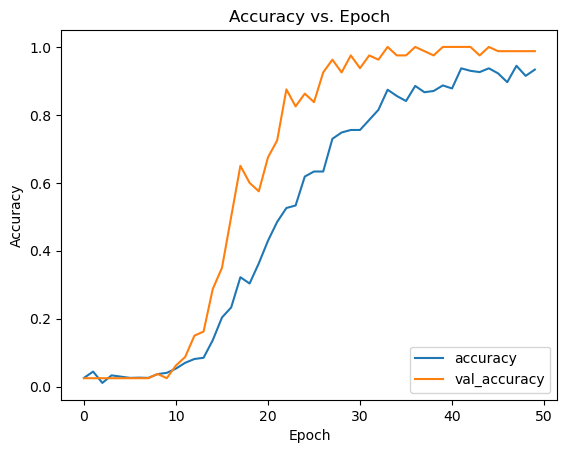
\includegraphics[width=3in]{cnn/1.png}
    \caption{Accuracy vs. Epochs}
    \label{fig:accuracy_vs_epoch}
\end{figure}

\subsection{Comparison between the models}

The comparison here \ref{tab:tab_comp_final} will be done with the best result from all models done in the previous section.

\begin{table}[ht!]
    \centering
    \caption{Classification - All Model} 
    \begin{tabular}{||c| c | c ||} 
    \hline
     ------ & Accuracy(Test) & Accuracy(Train) \\ [0.3ex] 
     \hline\hline
     Logistic Regression (HP/K-Fold) & 1.0 & 1.0\\
     \hline
    Gaussian Naive Bayes (HP/ K-Fold) & 0.975 &  0.997\\ 
    \hline
    SVM (Base Model/HP/ K-Fold) & 1.0 & 1.0 \\ 
    \hline
    K-NN (HP/K-Fold) & 0.938 & 1.0 \\ 
    \hline
    Decision Tree (K-Fold) & 0.650 & 0.906\\ 
    \hline
    LDA (Base Model/HP/ K-Fold) & 1.0 & 1.0\\ 
    \hline
    CNN  & 0.987 & 1.0\\ 
    \hline
    \end{tabular}
    \label{tab:tab_comp_final}
\end{table}

As we can see all models give us a great solution, apart Decision Tree, but we can consider the Logistic Regression and the SVM models the best, comparing the results with the others.

\section{Novelty and contributions}

We found two published articles that study the same problem as us, Performance Evaluation of Machine Learning Classifiers for Face Recognition \cite{9716171} and Face Recognition System Using Machine Learning Algorithm \cite{9137850}. The results obtained in the articles can be seen in the following tables \ref{tab:tab_performance_evaluation_article} \ref{tab:tab_Face_Recognition_System_article}.

\begin{table}[ht!]
    \centering
    \caption{Article Performance Evaluation results} 
    \begin{tabular}{||c| c ||} 
    \hline
     Machine Learning Model & Accuracy \\ [0.5ex] 
     \hline\hline
     PCA + Logistic Regression & 0.975 \\
     \hline
    PCA + Naïve Bayes & 0.950 \\ 
    \hline
    PCA + SVM & 0.988 \\ 
    \hline
    PCA + KNN & 0.888 \\ 
    \hline
    PCA + Decision Tree & 0.575\\ 
    \hline
    CNN & 0.988\\ 
    \hline
    \end{tabular}
    \label{tab:tab_performance_evaluation_article}
\end{table}

\begin{table}[ht!]
    \centering
    \caption{Article Face Recognition System results} 
    \begin{tabular}{||c| c ||} 
    \hline
     Machine Learning Model & Accuracy \\ [0.5ex] 
     \hline\hline
     PCA+Linear Discriminant Analysis & 1 \\
     \hline
    PCA + Naïve Bayes & 0.95 \\ 
    \hline
    PCA + SVM & 1 \\ 
    \hline
    \end{tabular}
    \label{tab:tab_Face_Recognition_System_article}
\end{table}

All our models give better, higher accuracy values than the paper Performance Evaluation of Machine Learning Classifiers for Face Recognition \cite{9716171} results. With paper Face Recognition System Using Machine Learning Algorithm \cite{9137850}, they give the same results, with the exception of Naïve Bayes which gives a slightly better result with our implemented solution.

Based on this analysis, we can say that we propose a better solution, with better performance of Machine Learning models.

\section{Conclusion}

Doing this project was very relevant since we not only successfully applied the machine learning algorithms learned in class, but we also self-learned new technics of machine learning using the internet. 
As we were developing our work, there were some periods where we found some difficulties, especially when we were dealing with data preprocessing and when we were implemented the CNN model. If we were to develop this work even further we would like to improve our data preprocessing. 
In conclusion, we can say that our best models are:Logistic Regression, LDA, and SVM with 100\% accuracy.
 In the end, we are very content with the work we presented, since it made us increase our knowledge.


\printbibliography

\end{document}
